\documentclass[10pt]{article}


\title{Transformers as Decision Makers: Provable In-Context Reinforcement Learning via Supervised Pretraining}

\date{\today}
\author{
  Licong Lin\thanks{UC Berkeley. Email: \texttt{liconglin@berkeley.edu}}\hspace{.35em}
  \and
  Yu Bai\thanks{Salesforce AI Research. Email: \texttt{yu.bai@salesforce.com}}\hspace{.35em}\footnotemark[4]
  \and
  Song Mei\thanks{UC Berkeley. Email: \texttt{songmei@berkeley.edu}}\hspace{.35em}\thanks{Equal contribution.}
}

\def\shownotes{0}  %set 1 to show author notes
\ifnum\shownotes=1
\newcommand{\authnote}[2]{{\scriptsize $\ll$\textsf{#1 notes: #2}$\gg$}}
\else
\newcommand{\authnote}[2]{}
\fi
\newcommand{\yub}[1]{{\color{red}\authnote{Yu}{#1}}}
\newcommand{\cfn}[1]
{{\color{blue}\authnote{Song}{#1}}}
\newcommand{\lc}[1]{{\color{blue}\authnote{Licong}{#1}}}
\newcommand{\todo}[1]{{\color{blue}$\ll$\textsf{\footnotesize TODO:
      {#1}$\gg$}}}

\makeatletter
\def\blfootnote{\gdef\@thefnmark{}\@footnotetext}
\makeatother

\begin{document}

\maketitle


\begin{abstract}
% In this project, we study using transformers to implement online bandit algorithms, with potential generalization to offline bandit and RL settings. 



Large transformer models pretrained on offline reinforcement learning datasets have demonstrated remarkable in-context reinforcement learning (ICRL) capabilities, where they can make good decisions when prompted with interaction trajectories from unseen environments. However, when and how transformers can be trained to perform ICRL have not been theoretically well-understood. In particular, it is unclear which reinforcement-learning algorithms transformers can perform in context, and how distribution mismatch in offline training data affects the learned algorithms. 
This paper provides a theoretical framework that analyzes supervised pretraining for ICRL. This includes two recently proposed training methods --- algorithm distillation and decision-pretrained transformers. First, assuming model realizability, we prove the supervised-pretrained transformer will imitate the conditional expectation of the expert algorithm given the observed trajectory. The generalization error will scale with model capacity and a distribution divergence factor between the expert and offline algorithms. Second, we show transformers with ReLU attention can efficiently approximate near-optimal online reinforcement learning algorithms like LinUCB and Thompson sampling for stochastic linear bandits, and UCB-VI for tabular Markov decision processes. This provides the first quantitative analysis of the ICRL capabilities of transformers pretrained from offline trajectories. 


% This paper theoretically investigates the supervised-pretraining approach that trains a transformer to predict an expert action given a query state and interaction trajectories. 


% In this paper, we provide a theoretical study of using transformers for in-context reinforcement learning (ICRL) with supervised pretraining. We show transformers can be used to implement online bandit algorithms like LinUCB, Thompson sampling, and UCB-VI. Our unified framework demonstrates supervised pretraining enables finding transformers that achieve competitive regret guarantees compared to expert algorithms.

% Specifically, we formally characterize regret bounds and transformer constructions when pretraining on different sources of expert actions, including algorithm distillation, optimal actions, and approximate optimal actions. Our analysis subsumes prior empirical works on algorithm distillation and decision transformer pretraining under a common theoretical lens.

% Overall, our results deliver fundamental insights on when and how supervised pretraining allows transformers to learn ICRL algorithms. We provide the first statistical and computational guarantees for using transformers as parametric decision makers that can efficiently adapt online in reinforcement learning contexts.
\end{abstract}
% \input{Sections/plans.tex}
\section{Introduction}

% \begin{itemize}[leftmargin=1.5em]
%     \item We theoretically show that transformers can do reinforcement learning in-context.~\yub{both statistical results and TF constructions are new. Previous paper (DPT) only analyzes minimizers under idealized assumptions.}
%     \item Namely, we prove that there exist TFs that can approximately implement LinUCB, Thompson sampling under the linear bandit setting (and maybe UCBVI under the MDP setting).
%     \item We use supervised pretraining (imitation learning) to find the TF. This idea appears in previous empirical works~\cite{laskin2022context,lee2023supervised}. \yub{Our statistical framework provides a unified framework that subsumes both AD and DPT.}
%     \yub{Can we say something about drawback of reward objective (instead of imitation)?}
%     \item We provide regret guarantees for the algorithm generated by the TF obtained vis supervised pretraining.
% \end{itemize}

The transformer architecture~\citep{vaswani2017attention} for sequence modeling has become a key weapon for modern artificial intelligence, achieving success in language~\citep{devlin2018bert,brown2020language,openai2023gpt} and vision~\citep{dosovitskiy2020image}. Motivated by these advances, the research community has actively explored how to best harness transformers for reinforcement learning (RL)~\citep{chen2021decision, janner2021offline, lee2022multi, reed2022generalist, laskin2022context, lee2023supervised,yang2023foundation}. While promising empirical results have been demonstrated, the theoretical understanding of transformers for RL remains limited. %\sm{deleted last sentence} Even fundamental questions such as \emph{approximation capabilities} (what algorithms in RL can be approximated by transformers) and \emph{sample efficiency} (how many samples are needed for training) remain largely open. 

%% Yu's original paragraph
% The transformer architecture~\citep{vaswani2017attention} for sequence modeling has become a key weapon for modern artificial intelligence. Motivated by their success in modalities such as language~\citep{devlin2018bert,brown2020language,openai2023gpt} and vision~\citep{dosovitskiy2020image}, how to best unleash their power for Reinforcement Learning (RL) has become an active research area, where various approaches have been proposed~\citep{chen2021decision, janner2021offline, lee2022multi, reed2022generalist, laskin2022context, lee2023supervised,yang2023foundation}. Despite promising empirical results, theoretical understandings on how to use transformers to do RL are still lacking---Even fundamental questions such as \emph{approximation} (what sequence-to-sequence functions in RL can be approximated by transformers) and \emph{statistical efficiency} (how many samples are needed to train such a transformer) remain largely open.


This paper provides theoretical insights into in-context reinforcement learning (ICRL)---an emerging approach that utilizes sequence-to-sequence models like transformers to perform reinforcement learning in newly encountered environments. In ICRL, the model takes as input the current state and past interaction history with the environment (the \emph{context}), and outputs an action. The key hypothesis in ICRL is that pretrained transformers can act as \emph{RL algorithms}, progressively improving their policy based on past observations. Approaches such as Algorithm Distillation \citep{laskin2022context} and Decision-Pretrained Transformers \citep{lee2023supervised} have demonstrated early successes, finding that \emph{supervised pretraining} can produce good ICRL performance. However, many concrete theoretical questions remain open about the ICRL capabilities of transformers, including but not limited to (1) what RL algorithms can transformers implement in-context; (2) what performance guarantees (e.g. regret bounds) can such transformers achieve when used iteratively as an online RL algorithm; and (3) when can supervised pretraining find such a good transformer. Specifically, this paper investigates the following open question:
\begin{center}
\emph{How can supervised pretraining on Transformers learn in-context reinforcement learning?}
\end{center}
% \yub{TODO: polish this question} \sm{changed "when" to "how"}


%% Yu's original paragraph
% This paper tackles this important open question in the scope of in-context reinforcement learning (ICRL)---An emerging approach for using sequence-to-sequence models (such as transformers) to perform RL in newly encountered environments. In ICRL, the model takes in the current state and past interaction history with the environment (the \emph{context}), and outputs an action. The underlying hypothesis in ICRL is that pretrained transformers can act as \emph{RL algorithms} that progressively improve their policy based on past observations. Approaches like Algorithm Distillation \citep{laskin2022context} and Decision-Pretrained Transformers \citep{lee2023supervised} demonstrated early successes in ICRL; in particular,  they find that \emph{supervised pretraining} can find transformers that perform good ICRL. However, many concrete theoretical questions remain open about the ICRL capabilities of transformers, including and not limited to (1) what RL algorithms can transformers implement in-context; (2) what performance guarantees (e.g. regret) can such transformers achieve when used iteratively as an online RL algorithm; and (3) when can supervised pretraining find such a good transformer. These motivate the following question:
% \begin{center}
% \emph{How can supervised pretraining on Transformers learn in-context reinforcement learning?}
% \end{center}




% Concretely, in ICRL, the transformer takes in a current state as well as a sequence of past interactions with an environment (such as a bandit or an MDP), which we call the \emph{context}, and is required to output an action. These approaches include the algorithm distillation (AD) approach \citep{laskin2022context} and decision-pretrained transformers (DPT) \citep{lee2023supervised} which demonstrated early successes. Specifically, these works find \emph{supervised pretraining} works well in finding good ICRL transformers. However, a more fundamental understanding is lacking of (1) what ICRL algorithms can the transformer architecture implement, (2) what regret guarantees they can obtain, and (3) when supervised pretraining works in finding such transformers. This motivates the following open question:
% \begin{center}
% \emph{When can supervised pretraining on Transformers learn in-context reinforcement learning?}
% \end{center}



% \yub{Finding expressive models for sequential decision making problems, such as RL, has been a central challenge, with modern architectures involving neural nets obtaining many successes.}~\yub{Sequence models, such as transformers for RL has been explored more recently (cite DT, AD, DPT, and also the review papers for FMDM).}~\yub{Despite the progress, how to best utilize sequence models to do powerful RL remains not well-understood in theory, and is still an active research area.}

% \yub{NOTE: There are two motivations for ICRL with sequence models: 1. find good architectures for decision making; 2. learn a model to do fast adaptation to new tasks (e.g. meta-RL~\citep{wang2016learning}). Right now, I am using 1 to motivate, but 2 may be a more concrete objective.}

% % ~\yub{The basic premise is that sequence models / Transformers can express more sophisticated target functions than their non-sequence counterparts.}

% \yub{A recent line of work proposes to use Transformers to do in-context reinforcement learning (ICRL), in which case TF aims to play in an unseen environment based on a handful of interations with this environment.} \yub{Concretely, in ICRL, the transformer takes in a current state as well as a sequence of past interactions with an environment (such as a bandit or an MDP) which we call the \emph{context}, and is required to output an action.}~\yub{This approach (ICRL) has been recently studied in the works of AD and DPT who showed some early success...}~\yub{Specifically, they find \emph{supervised pretraining} works well in finding such TFs.}~\yub{and they establish some preliminary theory such as such as connections to PS (maybe not needed)}~\yub{\textbf{However, a more fundamental understanding is lacking on (1) what ICRL algorithms can the transformer architecture implement, (2) what guarantees (e.g. regret) can they obtain, and (3) when supervised pretraining works in finding such transformers.}} This motivates the following open question:
% \begin{center}
% \emph{When can supervised pretraining on Transformers learn in-context reinforcement learning?}
% \end{center}


In this paper, we initiate a theoretical study of the ICRL capability of transformers under supervised pretraining to address the open questions outlined above. We show that (1) Transformers can implement prevalent RL algorithms, including LinUCB and Thompson sampling for stochastic linear bandits, and UCB-VI for tabular Markov decision processes; (2) The algorithms learned by transformers achieve near-optimal regret bounds in their respective settings; (3) Supervised pretraining find such algorithms as long as the sample size scales with the covering number of transformer class and distribution ratio between expert and offline algorithms. %\lc{offline or context algorithm?}

\paragraph{Summary of contributions and paper outline}
\begin{itemize}[leftmargin=1.5em]
\item We propose a general framework for supervised pretraining approaches to meta-reinforcement learning (Section~\ref{sec:framework}). This framework encompasses existing methods like Algorithm Distillation \citep{laskin2022context}, where the expert and context algorithms are identical, as well as Decision-Pretrained Transformers \citep{lee2023supervised}, where the expert generates optimal actions for the MDP. It also includes approximate DPT variants where the expert estimates optimal actions from full interaction trajectories. 
\item We prove that the supervised-pretrained transformer will imitate the conditional expectation of the expert algorithm given the observed trajectory (Section~\ref{sec:supervised-pretraining}). The generalization error scales with both model capacity and a distribution ratio measuring divergence between the expert algorithm and the algorithm that generated offline trajectories. 

\item We demonstrate that transformers can effectively approximate several near-optimal reinforcement learning algorithms by taking observed trajectories as context inputs (Section~\ref{sec:ICRL}). Specifically, we show transformers can approximate LinUCB (Section~\ref{sec:LinUCB-statement}) and Thompson sampling algorithms (Section~\ref{sec:TS-statement}) for stochastic linear bandit problems, and UCB-VI (Section~\ref{sec:Tabular-MDP-statement}) for tabular Markov decision processes. Combined with the generalization error bound from supervised pretraining and regret bounds of these RL algorithms, this provides regret bounds for supervised-pretrained transformers. 
\item Preliminary experiments validate that transformers can perform ICRL in our setup (Section~\ref{sec:experiments}).
\item Technically, we prove efficient approximation of LinUCB by showing transformers can implement accelerated gradient descent for solving ridge regression (\cref{sec:pf_thm:approx_smooth_linucb}), enabling fewer attention layers than the vanilla gradient descent approach in \cite{bai2023transformers}. To enable efficient Thompson sampling implementation, we prove transformers can compute matrix square roots through the Pade decomposition (\cref{sec:pf_thm:approx_thompson_linear-formal}). These approximation results are interesting in their own right. 
\end{itemize}
% \yub{We have two main contributions, transformers and statistical framework. In main sections, we do statistical framework first. In contribution list here, shall we reverse the order and state TF first? (TF can do LinUCB)}
% \sm{Experiments? }~\yub{added}

% \paragraph{Related work} Our work is intimately related to the lines of work on meta-reinforcement learning, in-context learning, transformers for decision-making, and the approximation theory of transformers. Due to limited space, we discuss these related works in~\cref {sec:related-work}.

% \begin{itemize}
%     \item Framework (supervised pretraining; context algorithm, expert algorithm), instantiation to bandit and MDP. 
    
%     \item Algorithm (MLE) and statistical results. Variations (source of the expert algorithm). Talk about application to both bandit and MDP.
%     \yub{Maybe connections to imitation learning.}
    
%     \item Transformer constructions (bandit, MDP).

%     \yub{We have two main contributions, transformers and statistical framework. In main sections, we do statistical framework first. In contribution list here, shall we reverse the order and state TF first? (TF can do LinUCB)}
%     \item Experiments.

%     \sm{Approximation: AGD, matrix square root. }
% \end{itemize}

\subsection{Related work}\label{sec:related-work}

\paragraph{Meta-learning and meta-reinforcement learning} In-context reinforcement learning can be cast into the framework of meta-learning and meta-reinforcement learning \citep{schmidhuber1987evolutionary, schmidhuber1992learning, bengio1990learning, naik1992meta, ishii2002control, schaul2010metalearning, thrun2012learning}. More recently, a line of work focuses on meta-learn certain shared structures such as the dynamics of the shared tasks \citep{fu2016one, nagabandi2018learning}, a task context identifier \citep{rakelly2019efficient, humplik2019meta, zintgraf2019varibad}, exploration strategies \citep{gupta2018meta}, or the initialization of the network policy \citep{finn2017model, hochreiter2001learning, nichol2018first, rothfuss2018promp}. Theories for this last approach of model-agnostic meta-learning have been explored by \cite{wang2020global}. 

Our work focuses on a more agnostic approach to learning the learning algorithm itself \citep{wang2016learning, duan2016rl, dorfman2021offline, mitchell2021offline, li2020focal, pong2022offline, laskin2022context, lee2023supervised}. Among these works, \cite{wang2016learning, duan2016rl} focus on the online meta-RL setting with the training objective to be the total reward. Furthermore, \cite{dorfman2021offline, mitchell2021offline, li2020focal, pong2022offline} focus on offline meta-RL, but their training objectives differ from the cross entropy loss used here, requiring explicit handling of distribution shift. The supervised pretraining approach we consider is most similar to the algorithm distillation methods of \cite{laskin2022context} and the decision-pretrained transformers of \cite{lee2023supervised}. We provide quantitative sample complexity guarantees and transformer constructions absent from previous work. 


\paragraph{In-context learning}

The in-context learning (ICL) capability of pretrained transformers has gained significant attention since being demonstrated on GPT-3 \cite{brown2020language}. Recent work investigates why and how pretrained transformers perform ICL \citep{garg2022can, li2023transformers, von2023transformers, akyurek2022learning, xie2021explanation, bai2023transformers, 
zhang2023trained, ahn2023transformers, raventos2023pretraining}. In particular, \cite{xie2021explanation} propose a Bayesian framework explaining how ICL works. \cite{garg2022can} show transformers can be trained from scratch to perform ICL of simple function classes.  \cite{von2023transformers, akyurek2022learning, bai2023transformers} demonstrate transformers can implement in-context learning algorithms via in-context gradient descent, with \cite{bai2023transformers} showing transformers can perform in-context algorithm selection. \cite{zhang2023trained} studied training dynamics of a single attention layer for in-context learning of linear functions. Our work focuses on the related but distinct capability of in-context decision-making for pretrained transformers. 

\paragraph{Transformers for decision making} Besides the ICRL approach, recent work has proposed goal-conditioned supervised learning (GCSL) for using transformers to make decisions \citep{chen2021decision, janner2021offline, lee2022multi, reed2022generalist, brohan2022rt, shafiullah2022behavior, yang2023foundation}. In particular, Decision Transformer (DT) \citep{chen2021decision, janner2021offline} uses transformers to autoregressively model action sequences from offline data, conditioned on the achieved return. During inference, one queries the model with a desired high return. Limitations and modifications of GCSL have been studied in \cite{yang2022dichotomy, paster2022you, vstrupl2022upside, brandfonbrener2022does}. A key distinction between GCSL and ICRL is that GCSL treats the transformer as a policy, whereas ICRL treats it as an algorithm for improving the policy based on observed trajectories. 



\paragraph{Expressivity of transformers} The transformer architecture, introduced by \cite{vaswani2017attention}, has revolutionized natural language processing and is used in most recently developed large language models like BERT and GPT \citep{devlin2018bert, brown2020language}. The expressivity of transformers has been extensively studied~\citep{yun2019transformers, perez2019turing, hron2020infinite,yao2021self, bhattamishra2020computational, zhang2022unveiling, liu2022transformers, wei2022statistically, fu2023can, bai2023transformers, akyurek2022learning, von2023transformers}. Deep neural networks such as ResNets and transformers have been shown to efficiently approximate various algorithms, including automata \citep{liu2022transformers}, Turing machines \citep{wei2022statistically}, variational inference \citep{mei2023deep}, and gradient descent \citep{bai2023transformers, akyurek2022learning, von2023transformers}. Our work provides efficient transformer constructions that implement accelerated gradient descent and matrix square root algorithms, complementing existing expressivity results. 





\paragraph{Statistical theories of imitation learning} Our generalization error analysis adapts classical analysis of maximum-likelihood estimator \citep{geer2000empirical}. The error compounding analysis for imitation learning appeared in early works \citep{ross2011reduction, ross2010efficient}. More recent theoretical analyses of imitation learning also appear in \cite{rajaraman2020toward, rajaraman2021provably, rashidinejad2021bridging}. 



% \sm{Add} \lc{add "throughout the proof, we assume the small probability $\delta_0,\delta<1/2$" to somewhere in the paper.}



% \begin{itemize}
% \item Meta-learning: \cite{schmidhuber1987evolutionary, schmidhuber1992learning, bengio1990learning, naik1992meta, ishii2002control, schaul2010metalearning, thrun2012learning}. Reward maximization Meta-RL: \cite{wang2016learning}, \cite{duan2016rl}. Hyperparameter Meta-RL: \cite{hochreiter2001learning}, \cite{finn2017model}, \cite{nichol2018first}. Offline meta-RL \cite{dorfman2021offline}, \cite{mitchell2021offline}, \cite{li2020focal}, \cite{pong2022offline}. AD: \cite{laskin2022context}, DPT: \cite{lee2023supervised}. 

% \item ICL: \cite{brown2020language}, \cite{garg2022can}, \cite{von2023transformers}, \cite{li2023transformers}, \cite{akyurek2022learning}, \cite{xie2021explanation}. \cite{bai2023transformers}, \cite{zhang2023trained}, \cite{ahn2023transformers}, \cite{xie2021explanation}. 

% \item Transformers for DM: \cite{chen2021decision}, \cite{janner2021offline}, \cite{lee2022multi}, \cite{reed2022generalist}, \cite{brohan2022rt}, \cite{shafiullah2022behavior}. \cite{yang2023foundation}, \cite{yang2022dichotomy}, \cite{brandfonbrener2022does}. 
% \item Imitation learning: \cite{rajaraman2020toward, rashidinejad2021bridging}. Meta-RL theory \cite{wang2020global}. \sm{More imitation learning literature? }
% \end{itemize}


\section{Framework for In-Context Reinforcement Learning}\label{sec:framework}

% \yub{should this section be actually our contribution instead of prelim? (since we subsume AD and DPT) If so, we can remove ``prelim'' in title, and attract more attention to this section.}

% \paragraph{Decision making environment} 


Let $\cM$ be the space of decision-making environments, where each environment $\inst \in \cM$ shares the same number of rounds $\totlen$ and state-action-reward spaces $\{ \statesp_t,  \actionsp_t, \rewardsp_t \}_{t \in [\totlen]}$. Each $\inst = \{\transmodel_\inst^{t-1}, \rewmodel_\inst^t \}_{t \in [\totlen]}$ has its own transition model $\transmodel_\inst^t: \statesp_{t} \times \actionsp_{t} \to \Delta(\statesp_{t+1})$ (with $\statesp_0$, $\actionsp_0 = \{ \emptyset \}$ so $\transmodel_\inst^0(\cdot) \in \Delta(\statesp_1)$ gives the initial state distribution) and reward functions $\rewmodel_\inst^{t}: \statesp_{t} \times \actionsp_{t} \to \Delta(\rewardsp_t)$. We equip $\cM$ with a distribution $\prior \in \Delta(\cM)$, the environment prior. While this setting is general, we later give concrete examples taking $\cM$ as $\totlen$ rounds of bandits or $K$ episodes of $H$-step MDPs with $\totlen = K H$. 

\paragraph{Distributions of offline trajectories} We denote a partial interaction trajectory, consisting of observed state-action-reward tuples, by $\dset_t=\{(\state_1,\action_1,\reward_1),\ldots,(\state_t,\action_t,\reward_t)\} \in \trajsp_t = \prod_{s \le t} (\statesp_s \times \actionsp_s \times \rewardsp_s)$ and write $\dset = \dset_{\totlen}$ for short. An algorithm $\sAlg$ maps a partial trajectory $\dset_{t-1} \in \trajsp_{t-1}$ and state $\state_t \in \statesp_t$ to a distribution over the actions $\sAlg(\cdot | \dset_{t-1}, \state_t) \in \Delta(\actionsp_t)$. Given an environment $\inst$ and algorithm $\sAlg$, the distribution over a full trajectory $\dset_\totlen$ is fully specified: 
\begin{align*}
\textstyle \P_{\inst}^{\sAlg}(\dset_\totlen) =
\prod_{t=1}^{\totlen}\transmodel_{\inst}^{t-1}(\state_{t}|\state_{t-1},\action_{t-1}) \sAlg(\action_t|\dset_{t-1},\state_t)\rewmodel_{\inst}^t(\reward_t|\state_t,\action_t).
\end{align*}
% \lc{introduce $\transmodel^0_\inst$ ($\state_1\sim\init$).} \sm{I added a parathesis in the paragraph above}
In supervised pretraining, we use a \textit{context algorithm} $\sAlg_0$ (which we also refer to as the offline algorithm) to collect the offline trajectories $\dset_\totlen$. For each trajectory $\dset_\totlen$, we also assume access to expert actions $\eaction = ( \eaction_t \in \actionsp_t )_{t \in \totlen} \sim \sAlg_{\shortexp}(\cdot | \dset_\totlen, \inst)$, sampled from an expert algorithm $\sAlg_{\shortexp}: \trajsp_\totlen \times \inst \to \prod_{t \in [\totlen]} \Delta(\actionsp_t)$. This expert could omnisciently observe the full trajectory $\dset_\totlen$ and environment $\inst$ to recommend actions. Let $\adset_\totlen = \dset_\totlen \cup \{ \eaction \}$ be the augmented trajectory. Then we have
\begin{align*}
\textstyle \P^{\sAlg_0,\sAlg_{\shortexp}}_{\inst}(\adset_\totlen)=\P^{\sAlg_0}_{\inst}(\dset_\totlen)\prod_{t=1}^\totlen \sAlg_{\shortexp}^t (\eaction_t|\dset_{\totlen},\inst).
\end{align*}
We denote $\P^{\sAlg_0,\sAlg_\shortexp}_{\prior}$ as the joint distribution of $(\inst,\adset_\totlen)$ where $\inst \sim \prior$ and $\adset_\totlen \sim \P^{\sAlg_0,\sAlg_\shortexp}_{\inst}$, and $\P^{\sAlg_0}_{\prior}$ as the joint distribution of $(\inst,\dset_\totlen)$ where $\inst \sim \prior$ and $\dset_\totlen \sim \P^{\sAlg_0}_{\inst}$. 

% When the actions $\eaction = \{ \eaction_t \in \actionsp_t \}_{t \in \totlen} \sim \prod_{t = 1}^T \sAlg_\Par^t( \cdot | \trajsp_{t-1}, \state_t)$ are sampled from algorithms of transformers $\sAlg_\Par$, we write $\P^{\sAlg_0,\sAlg_\Par}_{\inst}(\adset_\totlen)=\P^{\sAlg_0}_{\inst}(\dset_\totlen)\prod_{t=1}^\totlen \sAlg_\Par^t (\eaction_t|\trajsp_{t-1}, \state_t )$. We further denote $\P_{\prior}^{\sAlg_0,\sAlg_\Par}$ to be the joint distribution of $(\inst,\adset_\totlen)$ when $\inst \sim \prior$ and $\adset_\totlen \sim \P^{\sAlg_0,\sAlg_\Par}_{\inst}$, and define $\P^{\sAlg_0}_{\prior}$ and $\P^{\sAlg_0,\sAlg_\shortexp}_{\prior}$ similarly. 


\paragraph{Three special cases of expert algorithms} We consider three special cases of the expert algorithm $\sAlg_{\shortexp}$, corresponding to three supervised pretraining setups:
\begin{itemize}[leftmargin=1.5em]
\item[(a)] {\it Algorithm distillation \citep{laskin2022context}. } The algorithm depends only on the partial trajectory $\dset_{t-1}$ and current state $\state_t$: $\sAlg_{\shortexp}^t(\cdot|\dset_{\totlen},\inst) = \sAlg_{\shortexp}^t(\cdot|\dset_{t-1},\state_t)$. For example, $\sAlg_{\shortexp}$ could be a bandit algorithm like the Uniform Confidence Bound (UCB). 
\item[(b)] {\it Decision pretrained transformer (DPT) \citep{lee2023supervised}. } The algorithm depends on the environment $\inst$ and the current state $s_t$: $\sAlg_{\shortexp}^t(\cdot|\dset_\totlen, \inst) = \sAlg_{\shortexp}^t(\cdot|s_t, \inst)$. For example,  $\sAlg_{\shortexp}$ could output the optimal action $\action^*_t$ in state $\state_t$ for environment $\inst$. 
\item[(c)]{\it Approximate DPT. } The algorithm depends on the full trajectory $\dset_{\totlen}$ but not the environment $\inst$: $\sAlg_{\shortexp}^t(\cdot|\dset_\totlen, \inst) =\sAlg_{\shortexp}^t(\cdot|\dset_\totlen)$. For example, $\sAlg_{\shortexp}$ could estimate the optimal action $\widehat \action^*_t$ from the entire trajectory $\dset_\totlen$. 
\end{itemize}  
For any expert algorithm $\sAlg_{\shortexp}$, we define its reduced algorithm where the $t$-th step is $$\osAlg_{\shortexp}(\cdot|\dset_{t-1},\state_t) := \E_\prior^{\sAlg_0}[\sAlg_{\shortexp}^t(\cdot|\dset_\totlen,\inst)|\dset_{t-1},\state_t].$$ The expectation on the right is over $\P_{\prior}^{\sAlg_0} ( \dset_\totlen, \inst |\dset_{t-1},\state_t) =\prior(\inst) \cdot \P_\inst^{\sAlg_0}(\dset_\totlen) / \P_\inst^{\sAlg_0}(\dset_{t-1},\state_t).$ Note that the reduced expert algorithm $\osAlg_{\shortexp}$ generally depends on the context algorithm $\sAlg_0$. However, for cases (a) and (b), $\osAlg_{\shortexp}$ is independent of the context algorithm $\sAlg_0$. Furthermore, in case (a), we have $\osAlg_{\shortexp}^t = \sAlg_{\shortexp}^t$. 

% When $\inst$ is generated from the prior distribution $\prior$, we denote the joint distribution of $(\inst,\dset_\totlen,\eaction)$  as $\P_{\prior}^{\sAlg_0,\sAlg_\Par}$. We define $\P^{\sAlg_0}_{\prior}(\inst,\dset_\totlen)$, $\P^{\sAlg_0,\sAlg_\shortexp}_{\prior}(\inst,\dset_\totlen,\eaction)$ in a similar way. We use the same notation for the joint distribution and its marginal distribution when there is no confusion, for example, $\P_\prior^{\sAlg_0,\sAlg_\Par}(\dset_\totlen,\eaction)$ denotes the marginal distribution of  $(\dset_\totlen,\eaction)$ in the distribution $\P_\prior^{\sAlg_0,\sAlg_\Par}(\inst,\dset_\totlen,\eaction)$. 


% In addition, if the expert algorithm coincides with the algorithm used to collect the trajectory $\sAlg_{\shortexp}=\sAlg_0$, we may simply set $\eaction_t=\action_t$ to avoid sampling twice. 

\begin{comment}
\sm{I will start from here.}

\subsection{General framework}
Suppose the data collected for pretraining have the following form:
\begin{itemize}[leftmargin=1.5em]
\item   Sample a problem instance $\inst\sim\prior$. The learner does not observe $\inst$. 
\item Sample an interaction trajectory $D=\{(\state_1,\action_1,\reward_1),\ldots,(\state_\totlen,\action_\totlen,\reward_\totlen)\}$ with $\inst$ from context algorithm $\sAlg_0$. Concretely, $\state_i\in\statesp_t,\action_i\in\actionsp_t$ are the state and action selected at time $t$, where the state space $\statesp_t$ and action space $\actionsp_t$ are determined by $\inst$. $\reward_t$ is the observed reward   at time $t$ given $(\state_t,\action_t)$. 

Denote the distribution of the trajectory by $\P^{\sAlg_0}_{\inst}(\cdot)$. 
$\state_1$ is generated from $\P_{\inst,0}(\cdot)$. For each step $t\geq1$, given the history $\dset_{t-1}=\{(\state_1,\action_1,\reward_1),\ldots,(\state_{t-1},\action_{t-1},\reward_{t-1})\}$ and $\state_t$, the action $\action_t$ is sampled from the policy $\P^{\sAlg_0}_{\inst,t}(\cdot|\dset_{t-1},\state_t)=:\sAlg_0(\cdot|\dset_{t-1},\state_t)$. Given the action $\action_i$, we then  observe the reward $\reward_t\sim\P^r_{\inst,t}(\cdot|\state_t,\action_t
)$ and the next state $\state_{t+1}$ is  generated following the transition
$\P^s_{\inst,t}(\cdot|\state_t,\action_t)$. To sum up, we have (denoting $\P^s_{\inst,0}(\state_1|\state_0,\action_0)\defeq \P_{\inst,0}(\state_1)$)
\begin{align*}
\P_{\inst}^{\sAlg_0}(\dset_\totlen) =
\prod_{t=1}^{\totlen}\P^s_{\inst,t-1}(\state_{t}|\state_{t-1},\action_{t-1}) \P_{\inst,t}^{\sAlg_0}(\action_t|\dset_{t-1},\state_t)\P^r_{\inst,t}(\reward_t|\state_t,\action_t).
% \P_{\inst,0}(\state_1) \Big[\prod_{t=1}^{\totlen-1}\P_{\inst,t}^{\sAlg_0}(\action_t|\dset_{t-1},\state_t)\P_{\inst,t}(\reward_t|\state_t,\action_t)\P_{\inst,t}(\state_{t+1}|\state_{t},\action_t)\Big]\P_{\inst,\totlen}^{\sAlg_0}(\action_\totlen|\dset_{\totlen-1},\state_\totlen)\P_{\inst,\totlen}(\reward_\totlen|\state_\totlen,\action_\totlen).
\end{align*}
\item In addition to the interaction trajectory, at each step $t\geq 1$, an action $\eaction_t\in\actionsp_t$ is also generated from an expert algorithm (policy) $\sAlg_{\shortexp}$ with probability $\P^{\sAlg_{\shortexp}}_{\inst,t}(\cdot|\dset_{\totlen},\inst)$. Some special cases we consider are 
\begin{itemize}
\item $\P^{\sAlg_{\shortexp}}_{\inst,t}(\cdot|\dset_{\totlen},\inst)=\P^{\sAlg_{\shortexp}}(\cdot|\dset_{t-1},\state_t)=:\sAlg_{\shortexp}(\cdot|\dset_{t-1},\state_t)$, where the policy only depends  on the  trajectory  up to time $t$. As an example, this contains online RL/bandit algorithms such as UCB.
\item $\P^{\sAlg_{\shortexp}}_{\inst,t}(\cdot|\dset_{\totlen},\inst)=\P^{\sAlg_{\shortexp}}(\cdot|s_t, \inst)=:\sAlg_{\shortexp}(\cdot|s_t, \inst)$. As an example, this can implement the (ground truth) optimal action $\action^*_t$ at state $s_t$ in in $M$.
\item $\P^{\sAlg_{\shortexp}}_{\inst,t}(\cdot|\dset_{\totlen},\inst)=\P^{\sAlg_{\shortexp}}(\cdot|\dset_\totlen)=:\sAlg_{\shortexp}(\cdot|\dset_\totlen)$. As an example, this can implement the approximated (ground truth) optimal action $\widehat\action^*_t$ estimated from  the whole trajectory.
\end{itemize}  
Denote the dataset containing the trajectory and the addtional actions by $\adset_\totlen$. Then
\begin{align*}
\P^{\sAlg_0,\sAlg_{\shortexp}}_{\inst}(\adset_\totlen)=\P^{\sAlg_0}_{\inst}(\dset_\totlen)\prod_{t=1}^\totlen \P^{\sAlg_{\shortexp}}_{\inst,t}(\eaction_t|\dset_{\totlen},\inst).
\end{align*}
In addition, if the expert algorithm coincides with the algorithm used to collect the trajectory $\sAlg_{\shortexp}=\sAlg_0$, we may simply set $\eaction_t=\action_t$ to avoid sampling twice. 
\end{itemize}



\paragraph{Posterior averaging} 
For the second and the third case, we also define~\yub{important}
\begin{align*}
\sAlg_{\shortexp}(\cdot|\dset_{t-1},\state_t):=\E[\sAlg_{\shortexp}(\cdot|\dset_\totlen,\inst)|\dset_{t-1},\state_t], 
\end{align*}
where the expectation on the right hand side is taken over the posterior distribution
\begin{align*}
\P(\dset_\totlen,\inst|\dset_{t-1},\state_t) \; \propto_M \;
\prior(\inst)\cdot\P_\inst^{\sAlg_0}(\dset_{t-1},\state_t)\cdot\P_\inst^{\sAlg_0}(\dset_\totlen|\dset_{t-1},\state_t).
\end{align*}

\paragraph{Additional notation}
We use $\eaction=(\eaction_1,\ldots,\eaction_\totlen)$ to denote the additional actions selected following $\sAlg_{\Par}(\cdot|\dset_{t-1},\state_t)$ (or $\sAlg_{\shortexp}(\cdot|\dset_{t-1},\state_t)$) for $t\in[\totlen]$.
Given a problem instance $\inst$, let $\P^{\sAlg_0,\sAlg_\Par}_{\inst}$ denotes the joint distribution of the offline trajectory $\dset_\totlen$ and the actions selected $\eaction$.   If in addition $\inst$ is generated from the prior distribution $\prior$, we denote the joint distribution of $(\inst,\dset_\totlen,\eaction)$  as $\P_{\prior}^{\sAlg_0,\sAlg_\Par}$. We define $\P^{\sAlg_0}_{\prior}(\inst,\dset_\totlen)$, $\P^{\sAlg_0,\sAlg_\shortexp}_{\prior}(\inst,\dset_\totlen,\eaction)$ in a similar way. We use the same notation for the joint distribution and its marginal distribution when there is no confusion, for example, $\P_\prior^{\sAlg_0,\sAlg_\Par}(\dset_\totlen,\eaction)$ denotes the marginal distribution of  $(\dset_\totlen,\eaction)$ in the distribution $\P_\prior^{\sAlg_0,\sAlg_\Par}(\inst,\dset_\totlen,\eaction)$.  In all the results we assume the small probability $\delta<1/2$. \lc{this condition implies $\log(2/\delta)=O(\log(1/\delta))$.}

\end{comment}




































% \subsection{MDPs}

% \yub{Old framework below.}

% Data collection protocol for sampling a pretraining dataset $\Db$:
% \begin{itemize}
% \item Receive MDP instance $M\sim \Lambda$. The learner does not observe $M$.
% \item Sample interaction history (in-context dataset) $D = (\tau^1, \dots, \tau^T)$ from some distribution $\P^{\Alg_0}_M(D)$, where each $\tau^t=(s^t_1,a^t_1,r^t_1,\dots,s^t_H,a^t_H,r^t_H)$ is a trajectory from the MDP. This distribution admits the decomposition
% \begin{align*}
%     & \P^{\Alg_0}_M(D) = \prod_{t=1}^T \P_M(\tau^t) \paren{ \prod_{h=1}^H \Alg_0(a^t_h | s^t_h; \tau^t_{1:h-1}, D^{1:t-1}) }, \quad {\rm where} \\
%     & \P_M(\tau^t) = \prod_{h=1}^H \P_{M,h}(s^t_h|s^t_{h-1}, a^t_{h-1}) \RR_{M,h}(r^t_h | s^t_h, a^t_h).
% \end{align*}
% In typical cases where $\Alg_0$ predetermines a \emph{policy} $\pi^t\in\Pi$ before the $t$-th episode starts, we have (assuming $\pi^t$ is a Markov policy)
% \begin{align*}
%     \Alg_0(a^t_h | s^t_h; \tau^t_{1:h-1}, D^{1:t-1}) = \sum_{\pi^t\in\Pi} \Alg_0(\pi^t|D^{1:t-1}) \pi^t_h(a_h^t|s_h^t).
% \end{align*}

% \item Receive an ``expert action'' $\ab^t_h$ for each $(t,h)\in[T]\times[H]$:
% \begin{itemize}
%     \item (Option 1: Imitation) $\ab^t_h=(\ae_h)^t \sim \AlgE(\cdot | s^t_h; \tau^t_{1:h-1}, D^{1:t-1})$ from some expert algorithm $\AlgE$. A notable special case is $\Alg_0=\AlgE$ (on-policy case), where we can set $(\ae_h)^t=a_h^t$ for all $t\in[T]$ to avoid sampling twice. This was considered in the AD approach~\citep{laskin2022context}.
%     \item (Option 2: Optimal action) $\ab^t_h=a^{\star,t}_h\sim \pi^\star_{M,h}(\cdot|s_h^t)$ for the current MDP instance $M$. This was considered in the DPT approach~\citep{lee2023supervised}.
%     \item (Option 3: Approximate optimal action)~\yub{TBA}
% \end{itemize}
% Let $\Db\defeq(D, \sets{\ab^t_h}_{t,h\in[T]\times[H]})$ denote the interaction history augmented with the expert actions.
% \end{itemize}

% \begin{algorithm}[H]
% \caption{Supervised pretraining by MLE}
% \label{alg:mle-rl}
% \begin{algorithmic}[1]
% \REQUIRE Pretraining dataset $\Db^{(1:n)}$. MDP algorithm class $\sets{\pi_\btheta:\btheta\in\Theta}$.
% \STATE Solve the following MLE problem~\yub{no dependence on partial trajectory $\tau^t_{1:h-1}$}
% \begin{align*}
%     \hat{\btheta} = \argmax_{\btheta\in\Theta} \sum_{t=1}^T \sum_{h=1}^H \log \pi_\btheta(\ab_h^t | s_h^t; D^{1:t-1}).
% \end{align*}
% \ENSURE MDP algorithm $\hat{\btheta}$.
% \end{algorithmic}
% \end{algorithm}

% \paragraph{Results for imitation}
% Same as bandit case, since typical RL algorithms and our transformer constructions admit same protocols (which only use $D^{1:t-1}$ but not $\tau^t_{1:h-1}$).

% \yub{Copied from bandit}

% \begin{lemma}[Imitation; general case]
%     Under Option 1 (imitation), suppose there exists $\btheta^\star\in\Theta$ such that
%     \begin{align}
%     \label{eqn:pie-approximation}
%         \log\frac{\pi^E(\ae_t|o_t; D_{1:t-1})}{\pi_{\btheta^\star}(\ae_t|o_t; D_{1:t-1})} \le \eps
%     \end{align}
%     almost surely (under the above interaction protocol) for all $t\in[T]$. Then with probability at least $1-\delta$,~\cref{alg:mle-bandit} achieves
%     \begin{align*}
%         \E_{M\sim \Lambda, D^{1:t}\sim \P^{\Alg_0}_M}\brac{ \sum_{t=1}^T \HelDs\paren{ \pi_{\hat{\btheta}}(\cdot|o_t, D_{1:t-1}), \pi^E(\cdot|o_t, D_{1:t-1})} } \le \eps T + \cO\paren{ \log\paren{ \abs{\Theta} / \delta } }.
%     \end{align*}
% \end{lemma}

% \yub{We only need one-sided approximation, and only on $\ae_t$ (instead of all actions) in~\cref{eqn:pie-approximation}. Not really useful though.}
% \yub{Question: Can we weaken~\cref{eqn:pie-approximation} to some in-expectation version?}


% \paragraph{Results for fitting optimal actions}
% The theoretically optimal action can be recast as sampled from the following PS-full algorithm $\piPSf_\Lambda$. However, typically we only consider $\piPS_\Lambda$ (e.g. in RL theory).
% \begin{align*}
%     \piPSf_\Lambda(\cdot|s_h^t; \tau^t_{1:h-1}, D^{1:t-1}) &\defeq \E_{M\sim\Lambda, D^{1:t}\sim \P^{\Alg_0}_M}\brac{\pi^\star_{M,h}(\cdot|s_h^t) \mid \tau^t_{1:h-1}, D^{1:t-1}}, \\
%     \piPS_\Lambda(\cdot|s_h^t; D^{1:t-1}) &\defeq \E_{M\sim\Lambda, D^{1:t}\sim \P^{\Alg_0}_M}\brac{\pi^\star_{M,h}(\cdot|s_h^t) \mid D^{1:t-1}},
% \end{align*}

% \begin{lemma}[Bayesian approximation; general case]
%     Under Option 2 (optimal action), suppose there exists $\btheta^\star\in\Theta$ such that
%     \begin{align*}
%         \log\frac{\piPS_\Lambda(a^\star_t|s_h^t; D^{1:t-1})}{\pi_{\btheta^\star}(a^\star_t|s_h^t; D^{1:t-1})} \le \eps
%     \end{align*}
%     almost surely (under the above interaction protocol) for all $t\in[T]$. Then with probability at least $1-\delta$,~\cref{alg:mle-bandit} achieves
%     \begin{align*}
%         \E_{M\sim \Lambda, \tau\sim\P^{\Alg_0}_M}\brac{ \sum_{t=1}^T \sum_{h=1}^H \HelDs\paren{ \pi_{\hat{\btheta}}(\cdot|s_h^t; D^{1:t-1}), \piPS_\Lambda(\cdot|s_h^t; D^{1:t-1})} } \le \eps T H + \cO\paren{ \log\paren{ \abs{\Theta} / \delta } }.
%     \end{align*}
% \end{lemma}

% % {\color{red} Question: Need to bound both of the following terms
% % \begin{align*}
% %     \log\frac{\piPSf_\Lambda(a_h^{\star, t}|s_h^t; \tau^t_{1:h-1}, D^{1:t-1})}{\piPS_\Lambda(a_h^{\star, t}|s_h^t; \tau^t_{1:h-1}, D^{1:t-1})} ~~~{\rm and}~~~
% %     \log\frac{\piPS_\Lambda(a_h^{\star, t}|s_h^t; \tau^t_{1:h-1}, D^{1:t-1})}{\pi_{\btheta^\star}(a_h^{\star, t}|s_h^t; \tau^t_{1:h-1}, D^{1:t-1})}
% % \end{align*}
% % under the above interaction protocol.
% % }

\paragraph{Transformer architecture} We consider a sequence of $N$ input vectors $\set{\bh_i}_{i=1}^N\subset \R^D$, compactly written as an input matrix $\bH=[\bh_1,\dots,\bh_N]\in \R^{D\times N}$, where each $\bh_i$ is a column of $\bH$ (also a \emph{token}). Throughout this paper, we define $\sigma(t)\defeq \relu(t)=\max\sets{t,0}$ as the standard relu activation function. %\lc{add one sentence to explain why using relu instead of softmax is fine?}

% Decoder TFs are the same as encoder TFs, except that the attention layers are replaced by masked attention layers with a specific decoder-based (causal) attention mask.


\begin{definition}[Masked attention layer]
\label{def:masked-attention}
A masked attention layer with $M$ heads is denoted as $\Attn_{\btheta}(\cdot)$ with parameters $\btheta=\sets{ (\bV_m,\bQ_m,\bK_m)}_{m\in[M]}\subset \R^{D\times D}$. On any input sequence $\bH\in\R^{D\times N}$, we have $\bar{\bH} = \Attn_{\btheta}(\bH) = [\bar{\bh}_1, \ldots, \bar{\bh}_N] \in \R^{D \times N}$, where
% \begin{talign}
% \label{eqn:masked-attention}
%     \bar{\bH} = \Attn_{\btheta}(\bH)\defeq \bH + \sum_{m=1}^M (\bV_m \bH) \times \Big( (\MSK_{1:N',1:N'}) \circ \sursf\paren{ (\bQ_m\bH)^\top (\bK_m\bH) } \Big) \in \R^{D\times N'},
% \end{talign}
% where $\circ$ denotes the entry-wise (Hadamard) product of two matrices, and $\MSK \in \R^{N \times N}$ is the mask matrix given by 
% \[
% \MSK = \begin{bmatrix}
% 1 & 1/2 & 1/3 & \cdots & 1/N \\
% 0 & 1/2 & 1/3 & \cdots & 1/N\\
% 0 & 0 & 1/3 & \cdots & 1/N\\
% \cdots & \cdots & \cdots & \cdots & \cdots \\
% 0 & 0 & 0 & \cdots & 1/N
% \end{bmatrix}. 
% \]
% In vector form, we have
\begin{align*}
\textstyle    \bar{\bh}_i = \brac{\Attn_{\btheta}(\bH)}_i = \bh_i + \sum_{m=1}^M \frac{1}{i}\sum_{j=1}^i \barsig\paren{ \<\bQ_m\bh_i, \bK_m\bh_j\> }\cdot \bV_m\bh_j \in \R^D.
\end{align*}
\end{definition}

We remark that the use of ReLU attention layers is for technical reasons. In practice, both ReLU attention and softmax attention layers should perform well. Indeed, several studies have shown that ReLU transformers achieve comparable performance to softmax transformers  across a variety of tasks \citep{wortsman2023replacing, shen2023study, bai2023transformers}.

\begin{definition}[MLP layer]
\label{def:mlp}
An MLP layer with hidden dimension $D'$ is denoted as $\MLP_{\btheta}(\cdot)$ with parameters $\btheta=(\bW_1,\bW_2)\in\R^{D'\times D}\times\R^{D\times D'}$. On any input sequence $\bH\in\R^{D\times N}$, we have $\bar{\bH} = \MLP_{\btheta}(\bH) = [\bar{\bh}_1, \ldots, \bar{\bh}_N] \in \R^{D \times N}$, where
% $\MLP_{\btheta}(\bH)$ gives output
% \begin{talign*}
%     \bar{\bH} = \MLP_{\btheta}(\bH) \defeq \bH + \bW_2\barsig(\bW_1\bH),
% \end{talign*}
% where $\barsig: \R \to \R$ is the ReLU function. In vector form, we have 
\[
\bar{\bh}_i=\bh_i+\bW_2 \cdot \sigma(\bW_1\bh_i) \in \R^D.
\]
\end{definition}
We next define $L$-layer decoder-based transformers. Each layer consists of a masked attention layer (see Definition \ref{def:masked-attention}) followed by an MLP layer (see Definition \ref{def:mlp}) and a clip operation. 


% \begin{definition}[Clipped Transformer]
% \label{def:decoder-tf-clip}
% An $L$-layer decoder-based $\clipval$-clipped transformer, denoted as $\TF_\btheta^{\clipval}(\cdot)$, is a composition of $L$ self-attention layers, each followed by an MLP layer and a clip operation: $\bH^{(L)}=\TF_{\btheta}(\bH^{(0)})$, where $\bH^{(0)} = \clip_{\clipval}(\bH) \in\R^{D\times N}$ is the input sequence, and for $\ell\in\set{1,\dots,L}$, 
% \begin{talign*}
% \bH^{(\ell)} = \clip_{\clipval}\Big( \MLP_{\bthetamlp^{(\ell)}}\paren{ \Attn_{\bMAtt^{(\ell)}}\paren{\bH^{(\ell-1)}} } \Big),~~~~~ \clip_{\clipval}(\bh) = [\proj_{\| \bh \|_2 \le \clipval}(\bh_i)]_i. 
% \end{talign*}
% Above, the parameter $\btheta=(\bMAtt^{(1:L)},\bthetamlp^{(1:L)})$ consists of  $\bMAtt^{(\ell)}=\sets{ (\bV^{(\ell)}_m,\bQ^{(\ell)}_m,\bK^{(\ell)}_m)}_{m\in[M]} \subset \R^{D\times D}$ and  $\bthetamlp^{(\ell)}=(\bW^{(\ell)}_1,\bW^{(\ell)}_2)\in\R^{D' \times D}\times \R^{D\times D'}$.


\begin{definition}[Decoder-based Transformer]
\label{def:decoder-tf}
An $L$-layer decoder-based transformer, denoted as $\TF_\btheta^{\clipval}(\cdot)$, is a composition of $L$ masked attention layers, each followed by an MLP layer and a clip operation: $\TF_{\btheta}^{\clipval}(\bH) = \bH^{(L)} \in \R^{D \times N}$, where $\bH^{(L)}$ is defined iteratively by taking $\bH^{(0)} = \clip_{\clipval}(\bH) \in\R^{D\times N}$, and for $\ell\in [L]$, 
\begin{talign*}
\bH^{(\ell)} =\clip_{\clipval}\Big( \MLP_{\bthetamlp^{(\ell)}}\paren{ \Attn_{\bMAtt^{(\ell)}}\paren{\bH^{(\ell-1)}} } \Big) \in \R^{D \times N},~~~~~ \clip_{\clipval}(\bH) = [\proj_{\| \bh \|_2 \le \clipval}(\bh_i)]_i. 
\end{talign*}
Above, the parameter $\btheta=(\bMAtt^{(1:L)},\bthetamlp^{(1:L)})$ consists of  $\bMAtt^{(\ell)}=\sets{ (\bV^{(\ell)}_m,\bQ^{(\ell)}_m,\bK^{(\ell)}_m)}_{m\in[M]} \subset \R^{D\times D}$ and  $\bthetamlp^{(\ell)}=(\bW^{(\ell)}_1,\bW^{(\ell)}_2)\in\R^{D' \times D}\times \R^{D\times D'}$. We define the parameter class of transformers as $\Theta_{D, L, M, \hidden, B} \defeq \{ \btheta=(\bAtt^{(1:L)}, \bmlp^{(1:L)}): \nrmp{\btheta}\le B \}$, where the norm of a transformer $\TF_\btheta^{\clipval}$ is denoted as 
\begin{align}
\label{eqn:tf-norm}
    \nrmp{\btheta}\defeq \max_{\ell\in[L]} \Big\{  
    \max_{m\in[M]} \set{\lops{\bQ_m^\lth}, \lops{\bK_m^\lth} } + \sum_{m=1}^M \lops{\bV_m^\lth} +
    \lops{\bW_1^\lth} + \lops{\bW_2^\lth}
    \Big\}.
\end{align}
\end{definition}
We introduced clipped operations in transformers for technical reasons. For brevity, we will write $\TF_\btheta = \TF_\btheta^{\clipval}$ when there is no ambiguity. We will set the clipping value $\clipval$ to be sufficiently large so that the clip operator does not take effect in any of our approximation results.

%\sm{We allow $\clipval$ to be very large so that xxx}


% \begin{definition}[Decoder-based Transformer]
% \label{def:decoder-tf}
% An $L$-layer decoder-based transformer, denoted as $\TF_\btheta(\bH)$, is a composition of $L$ self-attention layers each followed by an MLP layer: $\bH^{(L)}=\TF_{\btheta}(\bH^{(0)})$, where $\bH^{(0)} = \bH \in\R^{D\times N}$ is the input sequence, and
% \begin{talign*}
% \bH^{(\ell)} = \MLP_{\bthetamlp^{(\ell)}}\paren{ \Attn_{\bMAtt^{(\ell)}}\paren{\bH^{(\ell-1)}} } \in \R^{D \times N},~~~\ell\in\set{1,\dots,L}.
% \end{talign*}
% Above, the parameter $\btheta=(\bMAtt^{(1:L)},\bthetamlp^{(1:L)})$ consists of  $\bMAtt^{(\ell)}=\sets{ (\bV^{(\ell)}_m,\bQ^{(\ell)}_m,\bK^{(\ell)}_m)}_{m\in[M]} \subset \R^{D\times D}$ and  $\bthetamlp^{(\ell)}=(\bW^{(\ell)}_1,\bW^{(\ell)}_2)\in\R^{D' \times D}\times \R^{D\times D'}$. We define the parameter class of transformers as $\Theta_{D, L, M, \hidden, B} \defeq \{ \btheta=(\bAtt^{(1:L)}, \bmlp^{(1:L)}): \nrmp{\btheta}\le B \}$, where the norm of a transformer $\TF_\btheta$ is denoted as 
% \begin{align}
% \label{eqn:tf-norm}
%     \nrmp{\btheta}\defeq \max_{\ell\in[L]} \Big\{  
%     \max_{m\in[M]} \set{\lops{\bQ_m^\lth}, \lops{\bK_m^\lth} } + \sum_{m=1}^M \lops{\bV_m^\lth} +
%     \lops{\bW_1^\lth} + \lops{\bW_2^\lth}
%     \Big\}.
% \end{align}
% %We will frequently consider ``\emph{attention-only}'' decoder-based transformers with $\bW_1^\lth,\bW_2^\lth=\bzero$, which we denote as $\TFz_\btheta(\cdot)$ for shorthand, with $\btheta=\btheta^{(1:L)}\defeq \bMAtt^{(1:L)}$.
% \end{definition}

% When we need to control the covering number of transformers $\{ \TF_\btheta: \btheta \in \Theta_{D, L, M, \hidden, B} \}$, we will consider the clipped transformer architecture, defined in Definition~\ref{def:decoder-tf-clip}. 




\paragraph{Algorithm induced by Transformers} We equip the transformer with an embedding mapping $\embedmap: \cup_{t \in [\totlen]} \statesp_t \cup \cup_{t \in [\totlen]} (\actionsp_t \times \rewardsp_t) \to \R^D$.  This assigns any state $\state_t \in \statesp_t$ a $D$-dimensional embedding vector $\embedmap(\state_t) \in \R^D$, and any action-reward pair $(\action_t, \reward_t) \in \actionsp_t \times \rewardsp_t$ a $D$-dimensional embedding $\embedmap(\action_t, \reward_t) \in \R^D$. The embedding function $\embedmap$ should encode the time step $t$ of the state, action, and reward. With abuse of notation, we denote $\embedmap(\dset_{t-1}, \state_t) = [\embedmap(\state_1), \embedmap(\action_1, \reward_1), \ldots, \embedmap(\action_{t-1}, \reward_{t-1}), \embedmap(\state_t)]$. We define a concatenation operator $\cat: \R^{D \times *} \to \R^{D \times *}$ that concatenates its inputs $\cat(\bh_1, \ldots, \bh_N) = [\bh_1, \ldots, \bh_N]$ in most examples, but it could also insert special tokens at certain positions (in MDPs we add an additional token at the end of each episode). For a partial trajectory and current state $(\dset_{t-1}, \state_t)$, we input $\bH = \cat(\embedmap(\state_1), \embedmap(\action_1, \reward_1), \ldots, \embedmap(\action_{t-1}, \reward_{t-1}), \embedmap(\state_t)) \in \R^{D \times *}$ into the transformer. This produces output $\bar{\bH} = \TF_{\btheta}^{\clipval}(\bH) = [\bar{\bh}_1, \bar{\bh}_2 \ldots, \bar{\bh}_{-2},\bar{\bh}_{-1}]$ with the same shape as $\bH$. To extract a distribution over the action space $\actionsp_t$ with $| \actionsp_t | = \Numact$ actions, we assume a fixed linear extraction mapping $\extractmap \in \R^{\Numact \times D}$. The induced algorithm is then defined as: $\sAlg_\btheta(\cdot | \dset_{t-1}, \state_t) = \softmax(\extractmap \cdot \bar{\bh}_{-1})$. The overall algorithm induced by the transformer is: 
\begin{equation}\label{eqn:transformer-algorithm}
\sAlg_\btheta(\cdot | \dset_{t-1}, \state_t) = \softmax ( {\extractmap} \cdot {\TF_\btheta^{\clipval}} ( {\cat}( {\embedmap} ( \dset_{t-1}, \state_t)))_{-1}). 
\end{equation}
We will always choose a proper concatenation operator $\cat$ in examples, so that in the pretraining phase, all the algorithm outputs $\{ \sAlg_\btheta(\cdot | \dset_{t-1}, \state_t) \}_{t \le \totlen}$ along the trajectory can be computed in a single forward propagation. 
\section{Statistical analysis of supervised pretraining}\label{sec:supervised-pretraining}
%That is, for each environment $\inst^\ith \sim_{iid} \prior$, an offline trajectory $\dset^\ith_\totlen$ is collected from the interaction of $\inst^\ith$ with $\sAlg_0$, augmented by expert actions $\eaction^\ith$ generated from $\sAlg_{\shortexp}$. Given a class of algorithms $\{ \sAlg_\Par \in \cup_{t \in [\totlen]} \{ (\trajsp_{t-1} \times \cS_t) \to \Delta(\actionsp_t) \}, ~\Par\in\Parspace\}$, supervised pretraining amounts to maximize the log-likelihood 

In supervised pretraining, we are given $\Numobs$ i.i.d offline trajectories $\{\dset^\ith_\totlen =  (\state^\ith_1,\action^\ith_1, \reward^\ith_1, \ldots, \state^\ith_\totlen, \allowbreak \action^\ith_\totlen, \allowbreak\reward^\ith_\totlen) \}_{i=1}^\Numobs \sim_{iid} \P_\prior^{\sAlg_0}$ from the interaction of $\inst^\ith \sim_{iid} \prior$ with an offline algorithm $\sAlg_0$. Given an expert algorithm $\sAlg_{\shortexp}$, we augment each trajectory $\dset_{\totlen}^i$ by $\{ \eaction_t^i \sim_{iid} \sAlg_{\shortexp}( \cdot |\dset_{t-1}^i, \state_t^i)\}_{t \in [\totlen]}$. Supervised pretraining maximizes the log-likelihood over the algorithm class $\{ \sAlg_\Par\}_{\Par\in\Parspace}$
\begin{align}
\EstPar=\argmax_{\Par\in\Parspace}  \frac{1}{\Numobs}\sum_{i=1}^\Numobs\sum_{t=1}^\totlen\log \sAlg_\Par(\eaction^\ith_{t}|\dset_{t-1}^\ith,\state^\ith_t). \label{eq:general_mle}
\end{align}
This section discusses the statistical properties of the algorithm learned via supervised pretraining. 

% When $\sAlg_\Par$ is specified by a transformer, this objective function coincides with the cross-entropy loss used to train transformers in supervised learning tasks. 
% where $\sAlg_\Par(\eaction^\ith_{t}|\dset_{t-1}^\ith,\state_t)$ denotes the probability of algorithm $\sAlg_\Par$ selects the action $\eaction^\ith_t$ given the historical trajectory $\dset_{t-1}^\ith$ and current state $\state^\ith_t$. 



\subsection{Main result}

% \yub{to be organized.}

% In this work, we will also apply the following standard concentration inequality (see e.g. Lemma A.4 in~\cite{foster2021statistical}).
% \begin{lemma}\label{lm:exp_concen}
%     For any sequence of random variables $(X_t)_{t\leq T}$ adapted to a filtration $\{\cF_{t}\}_{t=1}^T$, we have with probability at least $1-\delta$ that
%     \begin{align*}
%         \sum_{s=1}^t X_s\leq \sum_{s=1}^t\log\E[\exp(X_s)\mid\cF_{s-1}]+\log(1/\delta),~~~\text{for all } t\in[T].
%     \end{align*}
% \end{lemma}

Our main result demonstrates that the algorithm maximizing the supervised pretraining loss will imitate $\osAlg_{\shortexp}(\cdot|\dset_{t-1},\state_t) = \E_{\inst\sim \prior,  \dset_{\totlen} \sim \sAlg_0}[\sAlg_{\shortexp}^t(\cdot|\dset_\totlen,\inst)|\dset_{t-1},\state_t]$, the conditional expectation of the expert algorithm $\sAlg_{\shortexp}$ given the observed trajectory. The imitation error bound will scale with the covering number of the algorithm class and a  distribution ratio factor, defined as follows.

\begin{definition}[Covering number]\label{def:cover_number_general} For a class of algorithms $\{\sAlg_\Par,\Par\in\Parspace\}$, 
we say $\Parspace_0 \subseteq\Parspace$ is an  $\rho$-cover of $\Parspace$, if $\Parspace_0$ is a finite set such that for any $\Par\in\Parspace$, there exists $\Par_0\in\Parspace_0$ such that 
\[
\|\log \sAlg_{\Par_0}(\cdot|\dset_{t-1},\state_t)-\log \sAlg_{\Par}(\cdot|\dset_{t-1},\state_t)\|_{\infty}\leq\rho,~~~ \text{for all } \dset_{t-1},\state_t, t\in[\totlen].
\]
The covering number $\cN_{\Parspace}(\rho)$ is the minimal cardinality of $\Parspace_0$ such that $\Parspace_0$ is a $\rho$-cover of $\Parspace$.
\end{definition}

%\yub{Define covering number as sum of $t\in[T]$, then $T$ disappears in MLE rate?}



% \begin{lemma}[General guarantee for supervised pretraining]\label{lm:general_imit}
% Suppose Assumption~\ref{asp:realizability} holds. Then  the solution to~Eq.~\eqref{eq:general_mle} achieves
% \begin{align*}
% \E_{\dset_\totlen\sim \P^{\sAlg_0}_\prior}\brac{ \sum_{t=1}^\totlen \HelDs\paren{ \sAlg_{{\EstPar}}(\cdot|\dset_{t-1},\state_t ), \sAlg_{\shortexp}(\cdot|\dset_{t-1},\state_t )} } \le c\frac{\totlen \log \brac{ \cN_{\Parspace}(1/(\Numobs\totlen)^2) \totlen/\delta } }{n} + \totlen\geneps.
% \end{align*}
% with probability at least $1-\delta$ for some universal constant $c>0$.
% \end{lemma}
% See the proof in Section~\ref{sec:pf_lm:general_imit}. 



\begin{definition}[Distribution ratio]\label{def:dist_ratio}
\label{def:distribution-ratio}
We define the distribution ratio of two algorithms $\sAlg_1,\sAlg_2$ by
\begin{align*}\distratio_{\sAlg_1,\sAlg_2}
:=
\E_{\inst\sim\prior,\dset_\totlen\sim\P_\inst^{\sAlg_1}}
\Big[\prod_{s=1}^{\totlen}\frac{\sAlg_1(\action_s|\dset_{s-1},\state_s)}{\sAlg_2(\action_s|\dset_{s-1},\state_s)}\Big] = 1 + \chi^2\Big( \P_\prior^{\sAlg_1};\P_\prior^{\sAlg_2} \Big).
\end{align*}
\end{definition}

% \yub{This is chi-squared distance between the full trajectory under $\sAlg_1$ and $\sAlg_2$.}

Our main result requires the realizability assumption of algorithm class $\{ \sAlg_\Par\}_{\Par \in \Parspace}$ with respect to the conditional expectation of the expert algorithm. 

\begin{assumption}[Approximate realizability]
\label{asp:realizability}
% \lc{I think this includes both imitation and Bayes learning (PSfull). (Note that PS $=$ PSfull in bandit; later need another lemma  PS learning in MDPs).}
There exists $\TruePar\in\Parspace$ and $\geneps > 0$ such that for all $t\in[\totlen]$, 
\begin{align}
\label{eqn:plc_approx_general}
\log\E_{\inst \sim \prior, \adset_\totlen \sim \P_{\inst}^{\sAlg_0,\sAlg_\shortexp}}\Big[\frac{\osAlg_{\shortexp}(\eaction_t|\dset_{t-1},\state_t )}{\sAlg_\TruePar(\eaction_t|\dset_{t-1},\state_t )}\Big] \le \geneps. 
\end{align}
% where $\adset_\totlen$ follows the distribution  $\P_{\inst}^{\sAlg_0,\sAlg_\shortexp}$ with $\inst\sim\prior$. 
\end{assumption}
% It can be verified that a sufficient condition for Assumption~\ref{asp:realizability} is 
% \begin{align}\label{asp:realizability_suff}
% \log\frac{\osAlg_{\shortexp}(\eaction_t|\dset_{t-1},\state_t )}{\sAlg_\TruePar(\eaction_t|\dset_{t-1},\state_t )}\leq\geneps
% \end{align} almost surely over $\adset_\totlen\sim\P_{\inst}^{\sAlg_0,\sAlg_\shortexp},\inst\sim\prior$.  

% Let $\dset_\totlen=(\state_1,\action_1,\reward_1,\ldots,\state_\totlen,\action_\totlen,\reward_\totlen)$ denote a trajectory obtained by rolling out an algorithm $\sAlg$ in a problem instance $\inst$.  
% We define the (instance-dependent) expected cumulative reward\lc{maybe a different name?}
% \begin{align*}
% \textstyle \totreward_{\inst,\sAlg}(\totlen)
% :=\E_{\action\sim\sAlg}[\sum_{t=1}^\totlen \reward_t],
% \end{align*} where  the expectation is over the  states $\state_{t}\sim\P^s_{\inst,t}(\cdot|\state_{t-1},\action_{t-1})$, actions  $\action_t\sim\sAlg(\cdot|\dset_{t-1},\state_t)$ and rewards $\reward_t\sim\P^r_{\inst,t}(\cdot|\state_t,\action_t)$ for $t\in[\totlen]$.  

We aim to bound the performance gap between $\sAlg_{\EstPar}$ and $\sAlg_\shortexp$ in terms of expected cumulative rewards, where the expected cumulative reward is defined as 
\begin{align*}
\textstyle \totreward_{\prior,\sAlg}(\totlen)
:= \E_{\inst\sim\prior}\big[\totreward_{\inst,\sAlg}(\totlen) \big],~~~~~~~~~ \totreward_{\inst,\sAlg}(\totlen) = \E_{\dset_{\totlen} \sim\P^{\sAlg}_\inst}[\sum_{t=1}^\totlen \reward_t].
\end{align*}
An intermediate step of the result is controlling the expected Hellinger distance between two algorithms, where for distributions $p, q$, we have $\HelDs(p, q) = \int (\,\sqrt{p(x)} - \sqrt{q(x)} \,)^2 d x$. 

\begin{theorem}[Performance gap between expected cumulative rewards]\label{thm:diff_reward} Let Assumption~\ref{asp:realizability} hold and let $\EstPar$ be a solution to Eq.~\eqref{eq:general_mle}. Take $\distratio = \distratio_{\osAlg_\shortexp,\sAlg_0}$ as defined in Definition~\ref{def:dist_ratio}, and $\cN_{\Parspace} = \cN_{\Parspace}((\Numobs\totlen)^{-2})$  as defined in Definition~\ref{def:cover_number_general}. Then for some universal constant $c>0$, with probability at least $1-\delta$, we have 
%\lc{I still prefer the old version in statistical-proof.tex.}~
%\yub{$\geneps$ in separate sqrt?}
\begin{align}\label{eqn:Hellinger-bound-main-theorem}
&~ \E_{\dset_\totlen\sim \P^{\sAlg_\shortexp}_\prior}\Big[ \sum_{t=1}^\totlen \HelD \paren{  \sAlg_{{\EstPar}}(\cdot|\dset_{t-1},\state_t ),\osAlg_{\shortexp}(\cdot|\dset_{t-1},\state_t )} \Big] 
\le c {\totlen} \sqrt{\distratio}
\bigg(\sqrt{\frac{\log \brac{ \cN_{\Parspace} \cdot 
 \totlen/\delta } }{n}} +  \sqrt{\geneps}\bigg).
\end{align} 
Further assume that $|\reward_t| \leq 1$ almost surely. Then with probability at least $1-\delta$, the difference of the expected cumulative rewards between $\sAlg_\EstPar$ and $\osAlg_\shortexp$ satisfies
\begin{align}\label{eqn:reward-bound-main-theorem}
\Big|\totreward_{\prior,\sAlg_\EstPar}(\totlen)-\totreward_{\prior,\osAlg_\shortexp}(\totlen)\Big|
&\leq 
c \totlen^2 \sqrt{\distratio} \bigg(\sqrt{\frac{\log \brac{ \cN_{\Parspace} \cdot 
 \totlen/\delta } }{n}} +  \sqrt{\geneps}\bigg).
\end{align}
\end{theorem}

The proof of Theorem~\ref{thm:diff_reward} is contained in Section~\ref{sec:pf_thm:diff_reward}.

We remark that when the expectation on the left-hand-side of (\ref{eqn:Hellinger-bound-main-theorem}) is with respect to the measure $\P_\prior^{\sAlg_0}$, standard MLE analysis will provide a bound without the distribution ratio factor $\distratio = \distratio_{\osAlg_\shortexp,\sAlg_0}$ in the right-hand side. The distribution ratio factor arises from the distribution shift between trajectories generated by the expert algorithm $\sAlg_\shortexp$ versus the context algorithm $\sAlg_0$.  In addition, it should be noted that the result in Theorem~\ref{thm:diff_reward} holds generally provided Assumption~\ref{asp:realizability} is satisfied, which does not require that the algorithm class is induced by transformers.

% \sm{Can we provide an example in which reward maximization supervision is not the correct objective? }

% \yub{update statement to hellinger + total reward.} \yub{Strengthen the result to subsume the fast rate case when $C\approx 1$.} \sm{Discuss the distribution ratio. } \sm{Discuss the reward maximization pretraining objective. }



% \yub{Corollary: 1. AD; 2. DPT (comment on approximate DPT, or give another corollary box).}


\subsection{Implications in special cases}

\paragraph{Algorithm Distillation} When we set $\sAlg_\shortexp = \sAlg_0$, the supervised pretraining approach corresponds to the Algorithm Distillation method introduced in \cite{laskin2022context}. In this case, it suffices to set $\eaction^\ith = \action^\ith$ for every pretraining trajectory, eliminating the need to sample additional expert actions. The conditional expectation of the expert algorithm is given by $\osAlg_\shortexp = \sAlg_0$, and the distribution ratio $\distratio_{\sAlg_\shortexp,\sAlg_0}=1$. Under these conditions, Theorem~\ref{thm:diff_reward} ensures that $\sAlg_\EstPar$ imitates $\sAlg_0$ with a reward difference bounded by
\begin{align*}
\Big|\totreward_{\prior,\sAlg_\EstPar}(\totlen)-\totreward_{\prior,\sAlg_0}(\totlen)\Big|
&\leq c \totlen^2 \Big( \sqrt{\frac{\log \brac{ \cN_{\Parspace} \cdot \totlen/\delta } }{n} } + \sqrt{\geneps} \Big). 
\end{align*}
If the context algorithm $\sAlg_0$ does not perform well, we cannot expect the learned algorithm $\sAlg_\EstPar$ to have good performance, regardless of the number of offline trajectories. 
% For good performance of the learned algorithm $\sAlg_\EstPar$, it is crucial to have pretraining data generated by a high-quality context algorithm $\sAlg_0$. 

% The algorithm distillation approach studied in~\cite{laskin2022context} corresponds to the case when $\sAlg_\shortexp=\sAlg_0$. Under this setting, we have the distribution ratio $\distratio_{\sAlg_\shortexp,\sAlg_0}=1$ and Lemma~\ref{thm:diff_reward} provides the guarantee \begin{align*}
% |\totreward_{\prior,\sAlg_\EstPar}(\totlen)-\totreward_{\prior,\sAlg_\shortexp}(\totlen)|
% &\leq 
% c \genrewardb\cdot\totlen^2\sqrt{\frac{\log \brac{ \cN_{\Parspace}((\Numobs\totlen)^{-2}) \totlen/\delta } }{n} + \geneps}
% \end{align*}
% with probability at least $1-\delta$.  

\paragraph{Decision Pretrained Transformer} When we set $\sAlg_\shortexp^t = \sAlg_\shortexp^t(\state_t,\inst)=\action^*_t$ to be the optimal action at time $t$, the supervised pretraining approach corresponds to Decision-Pretrained Transformers (DPT) proposed in \cite{lee2023supervised}. In this case, the conditional expectation of the expert algorithm $\osAlg_\shortexp(\cdot|\dset_{t-1},\state_t)=\E[\sAlg_{\shortexp}(\cdot|\state_t,\inst)|\dset_{t-1},\state_t]=\sAlg_{\TS}(\cdot|\dset_{t-1},\state_t)$ is the Thompson sampling algorithm \citep[Theorem 1]{lee2023supervised}, which samples from the posterior distribution of the optimal action $\action^*_t$ given by $\P(a^*_t(\inst) |\dset_{t-1},\state_t)\propto \prior(\inst)\cdot\P_\inst^{\sAlg_0}(\dset_{t-1},\state_t)$. This implies that learning from optimal actions effectively learns to imitate Thompson sampling. Furthermore, the context algorithm is not required to perform well for the learned algorithm to be consistent with Thompson sampling. However, a high-quality context algorithm $\sAlg_0$ may help reduce the distribution ratio $\distratio$, thereby learning Thompson sampling with fewer samples. 


% The decision-pretrained transformer in~\cite{lee2023supervised} corresponds to the case  where the expert $\sAlg_\shortexp=\sAlg_\shortexp(\state_t,\inst)=\action^*_t$ gives the optimal action at time $t$. Therefore, the expert policy $\sAlg_\shortexp(\cdot|\dset_{t-1},\state_t)=\E[\sAlg_{\shortexp}(\cdot|\state_t,\inst)|\dset_{t-1},\state_t]=\sAlg_{\TS}(\cdot|\dset_{t-1},\state_t)$ equals the policy of Thompson sampling (i.e., the distribution of the optimal action $\action^*_t$  under the posterior $\P(\inst|\dset_{t-1},\state_t)\propto \prior(\inst)\cdot\P_\inst^{\sAlg_0}(\dset_{t-1},\state_t)$). This implies that learning from the optimal actions is effectively learning to imitate the Thompson sampling algorithm.



\paragraph{Approximate DPT} In practical scenarios, the learner may not have access to the optimal action $\action^*_t$ of the environment $\inst$ during pretraining. Instead, they might rely on an estimated optimal action $\widehat\action_t^* \sim \sAlg_{\shortexp}^t(\cdot | \dset_\totlen)$, derived from the entire trajectory $\dset_\totlen$. We can offer a guarantee analogous to Theorem~\ref{thm:diff_reward}, provided the distribution of the estimated action closely aligns with its posterior distribution: 
\begin{align}\E_{\dset_\totlen\sim\P_{\prior}^{\sAlg_0}}\KL{\sAlg_{\shortexp}^t(\cdot | \dset_\totlen)}{\P_{\TS,t}(\cdot|\dset_\totlen)}\leq\appeps,~~~ \forall t \in [\totlen]. 
\label{eq:app_opt_cond}
\end{align}
Here, $\P_{\TS,t}(\cdot|\dset_\totlen)$ represents the posterior distribution of the optimal action $\action^*_t=\action^*_t(\inst)$ at time $t$, given the observation $\dset_\totlen$, where $(\inst, \dset_\totlen) \sim \P_\prior^{\sAlg_0}$. 

% Note that in practice the learner may not know the optimal action $\action^*_t$ during pretraining, and may use an estimated optimal action $\widehat\action_t^*=\widehat\action^*_t(\dset_\totlen)$ as a surrogate. It can be shown that a similar guarantee as in Lemma~\ref{thm:diff_reward} can be established if the approximation error \begin{align}\E_{\dset_\totlen\sim\P_{\prior}^{\sAlg_0}}\KL{\widehat\action^*_t}{\P_{\TS,t}(\cdot|\dset_\totlen)}\leq\appeps
% \label{eq:app_opt_cond}
% \end{align} for all $t\in[\totlen]$ and some small $\appeps>0$, where $\P_{\TS,t}$ is the distribution of the optimal action $\action^*_t$ under the posterior $\inst|\dset_\totlen$. Note that  the error term $\appeps$  characterizes  the distance between the approximated optimal action $\widehat\action^*_t$ and the best guess we have about $\action^*_t$ given $\dset_\totlen$. \lc{Should put the result to appendix later}

\begin{proposition}\label{prop:app_opt_diff_reward} Let Assumption~\ref{asp:realizability} hold and let $\EstPar$ be the solution to Eq.~\eqref{eq:general_mle}. Take $\distratio = \distratio_{\sAlg_\TS,\sAlg_0}$ as defined in Definition~\ref{def:dist_ratio}, and $\cN_{\Parspace} = \cN_{\Parspace}((\Numobs\totlen)^{-2})$  as defined in Definition~\ref{def:cover_number_general}. Assume that for each trajectory, an estimated optimal action is provided $\widehat\action_t^* \sim \sAlg_{\shortexp}^t(\cdot | \dset_\totlen)$ at each time $t\in[\totlen]$ satisfying Eq.~\eqref{eq:app_opt_cond}. 
% Then for some universal constant $c>0$, with probability at least $1-\delta$, we have
% \begin{align*}
% &~  \E_{\dset_\totlen\sim \P^{\sAlg_\TS}_\prior} \Big[ \sum_{t=1}^\totlen \HelD \paren{ \sAlg_{{\EstPar}}(\cdot|\dset_{t-1},\state_t ), \sAlg_{\TS}(\cdot|\dset_{t-1},\state_t )} \Big] \\
% \le&~ c{\totlen} \sqrt{\distratio}
% \sqrt{\frac{\log \cN_{\Parspace} +\log(\totlen/\delta)}{n}+\geneps+\appeps}. 
% \end{align*}
% with probability at least $1-\delta$ for some universal constant $c>0$. 
Assume that the rewards $|\reward_t|\leq 1$  almost surely. Then for some universal constant $c>0$, with probability at least $1-\delta$, the difference of the expected cumulative rewards between $\sAlg_\EstPar$ and $\sAlg_\TS$ satisfies 
\begin{align*}
|\totreward_{\prior,\sAlg_\EstPar}(\totlen)-\totreward_{\prior,\sAlg_\TS}(\totlen)|
&\leq 
c \sqrt{\distratio}\cdot\totlen^2 \Big( \sqrt{\frac{\log \brac{ \cN_{\Parspace} \cdot \totlen/\delta } }{n} } + \sqrt{\geneps} + \sqrt{\appeps} \Big). 
\end{align*}
\end{proposition}
The proof of Proposition~\ref{prop:app_opt_diff_reward} is contained in Appendix~\ref{app:proof-prop-diff-reward-app-opt}. 




% Next, we choose the class of algorithms $\{\sAlg_\Par,\Par\in\Parspace\}$ to be algorithms induced by transformers. We show that such classes of algorithms has the potential to imitate state-up-the-art algorithms in  bandits and Markov Decision Processes (MDPs) settings. As a consequence, the algorithms we derived from transformers also have benign regret guarantee


\section{Approximation by transformers}\label{sec:ICRL}

In this section, we demonstrate the capability of transformers to implement prevalent reinforcement learning algorithms that produce near-optimal regret bounds. Specifically, we illustrate the implementation of LinUCB for stochastic linear bandits in Section~\ref{sec:LinUCB-statement}, Thompson sampling for stochastic linear bandits in Section~\ref{sec:TS-statement}, and UCB-VI for tabular Markov decision process in Section~\ref{sec:Tabular-MDP-statement}. %\sm{Add explanations of $\conO$, $\cO$, $\tcO$}

\subsection{LinUCB for linear bandits}\label{sec:LinUCB-statement}

A stochastic linear bandit environment is defined by $\inst=(\TrueLBPar,\Noisedist,\aset_1,\ldots,\aset_\totlen)$. For each time step $t\in[\totlen]$, the learner chooses an action $\action_t\in\R^{d}$ from a set of actions $\sA_t=\{\ba_{t,1},\ldots,\ba_{t,\Numact}\}$, which consists of $\Numact$ actions and may vary over time. Upon this action selection, the learner receives a reward $\reward_t=\<\action_t,\TrueLBPar\>+\Noise_t$. Here,$\{ \Noise_t \} \sim_{ iid} \Noisedist$ are zero-mean noise variables, and $\TrueLBPar\in\R^{d}$ represents an unknown parameter vector. Stochastic linear bandit can be cast into our general framework by setting $s_t = \aset_t$ and adopting a deterministic transition where $s_t$ transits to $s_{t+1}$ deterministically regardless of the chosen action. 



% Consider a class of linear bandit problems, in which at time $t\in[\totlen]$ the learner selects an action $\action_t\in\R^{d}$ from an action set $\sA_t=\{\ba_{t,1},\ldots,\ba_{t,\Numact}\}$ that consists of $\Numact$ actions, and observe the reward $\reward_t=\<\action_t,\TrueLBPar\>+\Noise_t$, where $\Noise_t\sim\Noisedist$ are i.i.d. zero mean noise and $\TrueLBPar\in\R^{d}$ is the unknown parameter vector. We allow the action sets $\aset_t$ to be vary across $t\in[\totlen]$. Note that the linear bandit instance is specified by $\inst=(\TrueLBPar,\Noisedist,\aset_1,\ldots,\aset_\totlen)$. To cast the linear bandit problem into our general framework, we assume $\inst$ follows the prior $\prior$ and let the state $\state_t=\aset_t$ for all $t\in[\totlen]$. Therefore, given the instance $\inst$, there exists only one possible state at each time $t$. 

% We now demonstrate that transformers are able to approximate  LinUCB~\cite{chu2011contextual}. 
We assume the context algorithm $\sAlg_0$ is the soft LinUCB \citep{chu2011contextual}. Specifically, for each time step $t\in[\totlen]$, the learner estimates the parameter $\TrueLBPar$ using linear ridge regression $\bw^t_{\ridge,\lambda}:=\argmin_{\bw\in\R^d} \sum_{j=1}^{t-1}(\reward_j-\<\ba_j,\bw\>)^2+ \lambda \|\bw\|_2^2$. Subsequently, the learner calculates the upper confidence bounds for the reward of each action as $v^*_{tk}:=\langle \ba_{t,k},\bw^t_{\ridge,\lambda}\rangle +\cwid \cdot (\ba_{t,k}^\top (\lambda\id_d+\sum_{j=1}^{t-1}\action_j\action_j^\top)^{-1}  \ba_{t,k})^{1/2}$. Finally, the learner selects an action $\action_t$ according to probability $\{ p^*_{t,j} \}_{j \in [\Numact]} = \softmax(\{v^*_{tj}/\temp \}_{j \in [\Numact]})$ for some sufficiently small $\temp>0$. Note that the soft LinUCB $\sAlg_{\sLinUCB(\temp)}$ recovers LinUCB as $\temp\to 0$. 
%\lc{(shall we put this into appendix?) }

% \begin{enumerate}
%     \item For some $\lambda>0$, computes  $\bw^t_{\ridge,\lambda}:=\argmin_{\bw\in\R^d}\frac{1}{2t}\sum_{j=1}^{t-1}(r_j-\<\ba_j,\bw\>)^2+\frac{\lambda}{2t}\|\bw\|_2^2$.
%     \item For each action $k\in[\Numact]$, computes $v^*_{tk}:=\<\ba_{t,k},\bw^t_{\ridge,\lambda}\>+\cwid\sqrt{\ba_{t,k}^\top \bA_{i}^{-1}  \ba_{t,k}}$ for some $\cwid$, where $\bA_t=\lambda\id_d+\sum_{j=1}^{t-1}\ba_j\ba_j^\top$.
%     \item Selects the action $\ba_{t,j}$ with probability $p^*_{t,j}=\frac{\exp(v^*_{tj}/\temp)}{\sum_{j=1}^\Numact\exp(v^*_{tk}/\temp)}$ for $j\in[\Numact]$ for some sufficiently small $\temp>0$.
% \end{enumerate} 

We further assume the existence of constants $\sigma,b_a,B_a,B_w>0$ such that the following conditions hold:   $|\Noise_t|\leq\sigma$, $b_a\leq\ltwo{\ba_{t,k}}\leq B_a$, and $\ltwo{\bw^*}\le B_w$ for all $t\in[\totlen],k\in[\Numact]$. Given these, the confidence parameter is defined as: $\cwid=\sqrt{\lambda}B_w+\sigma\sqrt{2\log (2B_aB_w \totlen )+d\log((d\lambda+\totlen B_a^2)/(d\lambda))} = \tcO(\sqrt{d})$. The following result shows that the soft LinUCB algorithm can be efficiently approximated by transformers, for which the proof is contained in Appendix~\ref{sec:pf_thm:approx_smooth_linucb}. 

\begin{theorem}[Approximating the soft LinUCB]\label{thm:approx_smooth_linucb}
Consider the embedding mapping $\embedmap$, extraction mapping $\extractmap$, and concatenation operator $\cat$ as in \ref{sec:tf_embed_bandit}. For any small $\eps,\temp>0$, there exists a transformer $\TF_\btheta^{\clipval}(\cdot)$ with $\log \clipval = \tcO(1)$, 
\begin{equation}
\begin{aligned}
&~D \le \conO(d\Numact),~ \layer=\tilde \cO(\sqrt{\totlen}),~ M \le 4\Numact,~D' = \tcO(d+A\sqrt{Td/(\temp\eps)}), ~\nrmp{\tfpar} = \tcO(\Numact+\totlen\sqrt{d}/(\temp\eps^{1/4})), \label{eq:linucb_tf_param} 
\end{aligned}
\end{equation}
such that taking $\sAlg_{\tfpar}$ as defined in Eq.~(\ref{eqn:transformer-algorithm}), we have
\[
\Big|\log \sAlg_{\sLinUCB(\tau)}(\ba_{t,k}|\dset_{t-1},\state_t) - \log \sAlg_{\tfpar}(\ba_{t,k}|\dset_{t-1},\state_t) \Big|\leq \eps, ~~~~\forall t\in[\totlen],k\in[\Numact].
\]
Here $\conO(\cdot)$ hides some absolute constant, and  $\tilde \cO(\cdot)$ additionally hides polynomial terms in $(\sigma, b_a^{-1}, B_a, B_w, \lambda^{\pm1})$, and poly-logarithmic terms in $(\totlen, \Numact, d, 1/\eps,1/\temp)$. 
\end{theorem}

% $\cO(\cdot)$ hides absolute constant and 
%\lc{not polynomial, but rational polynomials. Maybe do not mention this?} \lc{Also, this $D = \cO(d \Numact)$ is confusing, should be $D=O(d\Numact)$.  We have three things: universal constant, problem-dependent constant, logarithmic dependence.}

A key component in proving Theorem~\ref{thm:approx_smooth_linucb} is demonstrating that the transformer can approximate the accelerated gradient descent algorithm for solving linear ridge regression (Lemma~\ref{lm:approx_ridge}), a result of independent interest. Leveraging Theorem~\ref{thm:approx_smooth_linucb}, we can derive the following regret bound for the algorithm obtained via Algorithm Distillation, with the proof provided in Appendix~\ref{sec:pf_thm:smooth_linucb}.

\begin{theorem}[Regret of LinUCB and ICRL]\label{thm:smooth_linucb}
% Take  $0<\temp\leq\log(2\Numact B_a(B_w+2\alpha/\sqrt{\lambda}))/\sqrt{4\totlen}=\tilde O(1/\sqrt{\totlen})$, 
% the expected regret of the  smooth LinUCB satisfies 
%  \begin{align*}
%      \sum_{t=1}^\totlen\max_{k}\<\ba_{t,k},\bw^*\>-\totreward_{\inst,\sAlg_\sLinUCB}(\totlen)\leq\sqrt{8 d ({B_a}/{\sqrt{\lambda}}+1)^2T\alpha^2\log((d\lambda+TB_a^2)/(d\lambda))}+1+\sqrt{T}\leq Cd\sqrt{T}\log(T)
%  \end{align*}
% for some problem-dependent constant $C>0$ and all problem instance $\inst$. 
Let $\Theta = \Theta_{D, L, M, \hidden, B}$ be the class of transformers satisfying Eq.~\eqref{eq:linucb_tf_param} with $\eps=1/\totlen^3$ and $\temp = 1/ \log(4\totlen\Numact B_a(B_w+2\alpha/\sqrt{\lambda}))/\sqrt{4\totlen}=\tcO(\totlen^{-1/2})$, and choose the clip value $\log\clipval = \tcO(1)$. Let both the context algorithm $\sAlg_0$ and the expert algorithm $\sAlg_\shortexp$ coincide with the soft LinUCB algorithm $\sAlg_{\sLinUCB(\tau)}$ with parameter $\tau$ during supervised pretraining. Then with probability at least $1-\delta$, the learned algorithm $\sAlg_{\esttfpar}$, a solution to Eq.~\eqref{eq:general_mle}, entails the regret bound
\begin{align*}
\E_{\inst\sim\prior}\Big[\sum_{t=1}^\totlen\max_{k}\<\ba_{t,k},\bw^*\>-\totreward_{\inst,\sAlg_\esttfpar}(\totlen)\Big]&\leq   \cO\bigg( d\sqrt{\totlen}\log(\totlen)+ \totlen^2\sqrt{\frac{\log ( \cN_{\Parspace} \cdot \totlen/\delta )}{n} } \bigg),
% &\leq Cd\sqrt{T}\log(T)+\tilde O\Big(\totlen^2 \sqrt{\frac{\log(\Numobs/\delta)}{\Numobs}}\Big)
\end{align*}
where $\log \cN_{\Parspace} \le \tcO(\layer^2\embd(\head\embd+\hidden) \log\Numobs) \leq \tcO(\totlen^{3.5} d^2 \Numact^3\log\Numobs)$. Here $\cO$ hides polynomial terms in $(\sigma, b_a^{-1}, B_a, \\B_w, \lambda^{\pm1})$, and $\tcO$ additionally hides poly-logarithmic terms in $(\totlen, \Numact, d, 1/\eps,1/\temp)$. 
\end{theorem}

% \lc{do we want to hide $\log n$?}


\subsection{Thompson sampling for linear bandit}\label{sec:TS-statement}


We continue to examine the stochastic linear bandit framework of Section~\ref{sec:LinUCB-statement}, now assuming a Gaussian prior $\bw^\star\sim \cN(0,\Tpspar\id_d)$ and Gaussian noises $\{ \eps_t \}_{t \ge 0} \sim_{iid} \cN(0,\Tpsparn)$. Additionally, we assume existence of $(b_a, B_a)$ such that $b_a\leq\ltwo{\ba_{t,k}}\leq B_a$. In this model, Thompson sampling also utilizes linear ridge regression. Subsequently, we establish that transformers trained under the DPT methodology can learn Thompson sampling algorithms. We state the informal theorem in Theorem~\ref{thm:approx_thompson_linear} below, where its formal statement and proof are contained in Appendix~\ref{example:ts-app}. 

% \begin{theorem}[Approximating the Thompson sampling, Formal statement]\label{thm:approx_thompson_linear-formal}
% For any $0<\delta_0<1/2$, consider the same embedding mapping $\embedmap$ and extraction mapping $\extractmap$ as for soft LinUCB in \ref{sec:tf_embed_bandit},
% %\sm{Link}\lc{same as before},
% and consider the standard concatenation operator $\cat$. Under Assumption~\ref{ass:thompson_mlp_approx_linear},~\ref{ass:thompson_mlp_diff_action_linear}, for $\eps<(\Trunregp\wedge1)/4$, there exists a  transformer $\TF_\btheta(\cdot)$ with \sm{$\TF_\btheta^{\clipval}(\cdot)$ with $\log \clipval = \tcO(1)$?}
% \begin{align}
% &D=\tcO(T^{1/4}Ad),~L= \tcO(\sqrt{T}),~\sup_{l\in[L]}M^{\lth}=\tcO(AT^{1/4}),~\hidden=\tcO(A(T^{1/4}d+\neuron))~,\notag\\
% &~~~\nrmp{\btheta}\leq \tcO(T+AT^{1/4}+\sqrt{ \neuron A}+\weightn),\label{eq:ts_tf_param-formal}
% \end{align} 
% such that 
% $\log\frac{\sAlg_{\TS}(\action_t|\dset_{t-1},\state_t)}{\sAlg_{\tfpar}(\action_t|\dset_{t-1},\state_t)}\leq \eps$ for all $t\in[T],k\in[A]$ with probability at least $1-\delta_0$.  Here  
% $\neuron,\weightn$ are the values defined in   Assumption~\ref{ass:thompson_mlp_approx_linear} with $\trunprob=\eps/(4A),\Trunregpa=\Trunregp,\delta=\delta_0$, and $\tcO(\cdot)$ hides rational polynomial terms in $(\lambda,\Tpsparn,b_a,B_a)$ and logarithmic terms in $(\totlen,A,d,1/\delta_0,1/\eps)$.
% \end{theorem}

\begin{theorem}[Approximating the Thompson sampling, Informal]\label{thm:approx_thompson_linear}
Consider the embedding mapping $\embedmap$, extraction mapping $\extractmap$, and concatenation operator $\cat$ as in \ref{sec:tf_embed_bandit}. 
% Consider the same embedding mapping $\embedmap$ and extraction mapping $\extractmap$ as for soft LinUCB in \ref{sec:tf_embed_bandit}, and consider the standard concatenation operator $\cat$. 
Under Assumption~\ref{ass:thompson_mlp_approx_linear},~\ref{ass:thompson_mlp_diff_action_linear}, for sufficiently small $\eps$, there exists a transformer $\TF_\btheta^{\clipval}(\cdot)$ with $\log \clipval = \tcO(1)$, 
\begin{equation}\label{eq:ts_tf_param-main}
\begin{aligned}
&~D = \tcO(AT^{1/4}d),~~~~~ L=\tilde \cO(\sqrt{T}),~~~M =\tilde \cO(A T^{1/4}), \\
&~\nrmp{\btheta} = \tcO(T+A T^{1/4}+\sqrt{A}),~~~~~ \hidden = \tcO(A T^{1/4}d),
\end{aligned}
\end{equation}
such that taking $\sAlg_{\tfpar}$ as defined in Eq.~(\ref{eqn:transformer-algorithm}), with probability at least $1-\delta_0$ over $(\inst, \dset_{\totlen}) \sim \P_{\prior}^{\sAlg}$ for any $\sAlg$, we have
\[
 \log \sAlg_{\TS}(\ba_{t,k}|\dset_{t-1},\state_t) - \log \sAlg_{\tfpar}(\ba_{t,k}|\dset_{t-1},\state_t) \leq \eps,~~~~\forall t\in[T],k\in[A]. 
\]
Here, $\tcO(\cdot)$ hides polynomial terms in $(\neuron,\weightn, \Tpspar^{\pm1}, \Tpsparn^{\pm1}, b_a^{-1}, B_a)$, and poly-logarithmic terms in $(\totlen, \Numact, d, 1/\eps,\\ 1/\delta_0)$, where $(\neuron, \weightn)$ are parameters in Assumption~\ref{ass:thompson_mlp_approx_linear} and \ref{ass:thompson_mlp_diff_action_linear}. 
%Here $M,C$ are the values defined in   Assumption~\ref{ass:thompson_mlp_approx_linear} with $\trunprob=c\eps/K$ for some universal constant $c>0$, and $\tilde O(\cdot)$ hides logarithmic dependency on $\totlen,K,d,1/\delta_0,1/\eps$.\lc{the dependence on $M,C$ is written in terms of the dependence on other variables.}
\end{theorem}

Central to proving Theorem~\ref{thm:approx_thompson_linear} is establishing that the transformer can approximate matrix square roots via Pade decomposition (\cref{sec:pf_thm:approx_thompson_linear-formal}), a result of independent interest. Theorem~\ref{thm:approx_thompson_linear} thereby implies the subsequent regret bound for transformers trained under DPT. 

\begin{theorem}
[Regret of Thompson sampling and ICRL]\label{thm:ts_linear_regret}
% Let the distributional assumptions stated in Section~\ref{example:ts} holds. %Thompson sampling achieves the Bayes regret 
% \begin{align*}  \E_{\inst\sim\prior}\Big[\sum_{t=1}^\totlen\max_{k}\<\ba_{t,k},\bw^*\>-\totreward_{\inst,\sAlg_\TS}(\totlen)\Big]\leq Cd\sqrt{\totlen}\log(\totlen d)
% \end{align*}
% for some problem-dependent constant $C>0$. 
% Suppose in addition Assumption~\ref{ass:thompson_mlp_approx_linear},~\ref{ass:thompson_mlp_diff_action_linear} are in force. 
Follow the assumptions of Theorem~\ref{thm:approx_thompson_linear}. Let $\Theta = \Theta_{D, L, M, \hidden, B}$ be the class of transformers satisfying Eq.~\eqref{eq:ts_tf_param-main} with $\eps=1/(\distratio\totlen^3)$,   $\delta_0=\delta/(2n)$, and choose the clip value $\log \clipval = \tcO(1)$. Assume the trajectories are collected by some context algorithm $\sAlg_0$, and we choose the expert algorithm $\sAlg_\shortexp(\state_t,\inst)=\action^*_t=\argmax_{\ba\in\sA_t}\<\ba,\bw^*\>$ to be the optimal action of the bandit instance $\inst$ for each trajectory. Then with probability at least $1-\delta$, the learned algorithm $\sAlg_{\esttfpar}$, a solution to Eq.~\eqref{eq:general_mle}, entails regret bound
\begin{align*}
\E_{\inst\sim\prior}\Big[\sum_{t=1}^\totlen\max_{k}\<\ba_{t,k},\bw^*\>-\totreward_{\inst,\sAlg_\esttfpar}(\totlen)\Big]&\leq \cO \bigg( d\sqrt{T}\log(Td)+ \sqrt{\distratio} \cdot\totlen^2\sqrt{\frac{\log ( \cN_{\Parspace} \totlen/\delta ) }{n} } \bigg), 
\end{align*}
where $\distratio = \distratio_{\sAlg_\TS,\sAlg_0}$, and $\log \cN_{\Parspace} \le \tcO(\layer^2\embd(\head\embd+\hidden)\log \Numobs )  \leq\tcO(\totlen^{5/4}\Numact^2 d(\neuron+\Numact\sqrt{\totlen}d)\log\Numobs)$. Here $\cO$ hides polynomial terms in $(\Tpspar^{\pm1}, \Tpsparn^{\pm1}, b_a^{-1}, B_a)$, and $\tcO$ additionally hides poly-logarithmic terms in   $(\neuron,\weightn,\\~ \totlen, \Numact, d, 1/\eps, 1/\delta_0)$. 
\end{theorem}

% \lc{the $\delta_0=\delta/(2n)$ dependence is annoying. This means $\log(1/\delta)$ contains polylogarithmic terms in $n$... may need to redefine $\tcO(\cdot)$ to include $\log n$ terms?}\lc{Also, do we want to remove the term $\log(Td)$?}



\subsection{UCB-VI for Tabular MDPs}\label{sec:Tabular-MDP-statement}


A finite-horizon tabular MDP is specified by $\inst=(\statesp,\actionsp, \horizon, \{\transit_h\}_{h\in[\horizon]},\{\rewardfun_h\}_{h\in[\horizon]},\init)$, with $\horizon$ being the time horizon, $\statesp$ the state space of size $\Numst$, $\actionsp$ the action space of size $\Numact$, and $\init\in\Delta(\statesp)$ defining the initial state distribution. At each time step $h\in[\horizon]$, $\transit_h: \statesp\times\actionsp \to \Delta(\statesp)$ denotes the state transition dynamics and $\rewardfun_h:\statesp \times \actionsp \to [0,1]$ gives the reward function. A policy $\plc:=\{\plc_h:(\statesp \times\actionsp \times \R)^{h-1}\times\statesp \to\Delta(\actionsp)\}_{h \in [\horizon]}$ maps history and state to a distribution over actions. The value of policy $\pi$ interacting with environment $\inst$ is defined as the expected cumulative reward $\valuefun_\inst(\plc)=\E_{\inst,\plc}[\sum_{h=1}^\horizon \rewardfun_h (\state_h,\action_h)]$. A policy $\optplc$ is said to be optimal if $\optplc=\argmax_{\pi\in\Delta(\plcset)}\valuefun_\inst(\pi)$. 
%We use $\plcset$ to denote all possible deterministic policies,  and let $\Delta(\plcset)$ be either the set of all  policies or the set of all  distributions over the  deterministic policies. $\optplc$ is said to be an optimal policy if $\optplc=\argmax_{\pi\in\Delta(\plcset)}\valuefun_\inst(\pi)$. 


We let the context algorithm $\sAlg_0$ interact with an MDP instance $\inst$ to generate $\Numepi$ episodes, each consisting of $\horizon$ horizon sequences $ (\state_{k,h},\action_{k,h},\reward_{k,h})_{k \in [\Numepi], h \in [\horizon]}$. These can be reindexed into a single trajectory $\dset_{\totlen} = \{ (\state_t,\action_t,\reward_t) \}_{t \in [\totlen]}$ with $t=H(k-1)+h$ and $\totlen=\Numepi\horizon$. The Bayes regret of any algorithm $\sAlg$ gives $\E_{\inst\sim\prior}[\Numepi\Vfun_\inst(\plc^*)-\totreward_{\inst,\sAlg}(\totlen)]$. 
%We may view the whole interaction trajectory of length $\totlen$ as $\Numepi$ episodes from the finite-horizon MDP. For any $t\in[\totlen]$, write $t=H(k-1)+h$ for some and denote $\state_t,\action_t,\reward_t$ by $\state_{k,h},\action_{k,h},\reward_{k,h}$, respectively.

% \paragraph{The UCB-VI algorithm} 

Near minimax-optimal regret for tabular MDPs can be attained through the UCB-VI algorithm \citep{azar2017minimax}. We demonstrate that transformers are capable of approximating the soft UCB-VI algorithm $\sAlg_{\sUCBVI(\tau)}$, a slight modification of UCB-VI formalized in Appendix~\ref{sec:tf_embed_mdp}. 

% Namely, UCB-VI implements the following steps:

% for each episode $k\in[\Numepi]$ and each step $h=\horizon,\ldots,1$
% \begin{enumerate}
%     \item Compute the estimated transition matrix $\tresttransit_h(\state'|\state,\action):=   \frac{\Numvi_h(\state,\action,\state')}{\Numvi_h(\state,\action)\vee 1}$,  where $\Numvi_h(\state,\action,\state')$ denotes the number of times the state-action-next-state tuples has been visited in the first $k-1$ episodes, and $\Numvi_h(\state,\action)=\sum_{\state'}\Numvi_h(\state,\action,\state')$ (we assume $\Numvi_\horizon(\state,\action,\state')=0$ and $\Numvi_\horizon(\state,\action)$  be the number of times $(\state,\action)$ is visited at timestep $\horizon$).
%     \item Calculate the estimated Q-function \begin{align*}
% \trestQfun_h(\state,\action)=\min\{\horizon,\reward_h(\state,\action)+\bonus_h(\state,\action)+\sum_{\state'\in\statesp}\tresttransit_h(\state'\mid\state,\action)\trestVfun_{h+1}(\state')\},\end{align*}
% where the bonus $\bonus_h(\state,\action)=2\horizon\sqrt{\frac{\log(\Numst\Numact\totlen/\delta)}{\Numvi_h(\state,\action)\vee1}}$,  $\trestVfun_{\horizon+1}(\state):=0$ for all $\state\in\statesp$ and $\trestVfun_h(\state):=\max_{\action\in\actionsp}\trestQfun_h(\state,\action)$. 
% \end{enumerate}
% During policy execution, at each step $h\in[\horizon]$, UCB-VI takes the greedy action $\action_h:=\argmax_{\action}\trestQfun(\state_h,\action)$ and observes the reward and next state $(\reward_h,\state_{h+1})$. To facilitate pretraining, in this work we consider a smoothed version of UCB-VI, which takes action $\action_h$  following the softmax policy $\plc_h(\action|\state_h)=\frac{\exp(\trestQfun(\state_h,\action)/\temp)}{\lone{\exp(\trestQfun(\state_h,\action)/\temp)}}$ for some sufficiently small $\temp>0$. Note that the smoothed UCB-VI recovers UCB-VI as $\temp\to 0$.

\begin{theorem}[Approximating the soft UCB-VI]\label{thm:approx_ucbvi}
% Let $R=2\max\{(B_a+\alpha/\sqrt{\lambda})\}$.
Consider the embedding mapping $\embedmap$, extraction mapping $\extractmap$, and concatenation operator $\cat$ as in Appendix~\ref{sec:tf_embed_mdp}. There exists a transformer $\TF_\btheta^{\clipval}(\cdot)$ with $\log \clipval = \tcO(1)$, 
\begin{equation}\label{eq:ucbvi_tf_param-main}
\begin{aligned}
&~D =\conO(\horizon\Numst^2\Numact),~~~L= 2\horizon+8,~~~M= \conO(\horizon\Numst^2\Numact),\\
&~\hidden= \conO(\Numepi^2\horizon\Numst^2\Numact),~~~~\nrmp{\btheta}\leq \tcO(\Numepi^2\horizon\Numst^2\Numact+\Numepi^3+1/\temp),
\end{aligned} 
\end{equation}
such that 
$\sAlg_{\sUCBVI(\tau)}(\action|\dset_{t-1},\state_t) = \sAlg_{\tfpar}(\action|\dset_{t-1},\state_t)$ for all $t\in[T],\action\in\actionsp$. Here $\conO(\cdot)$ hides universal constants and $\tcO(\cdot)$  hides poly-logarithmic terms in $(\horizon,\Numepi,\Numst,\Numact,1/\temp)$. 
\end{theorem}

Leveraging Theorem~\ref{thm:approx_ucbvi}, we can derive the following regret bound for the algorithm obtained via Algorithm Distillation. 

\begin{theorem}[Regret of UCB-VI and ICRL]\label{thm:ucbvi_icrl-main}
Let $\Theta = \Theta_{D, L, M, \hidden, B}$ be the class of transformers satisfying Eq.~\eqref{eq:ucbvi_tf_param-main} with $\temp = 1/\Numepi$, and choose the clip value $\log \clipval = \tcO(1)$. Let both the context algorithm $\sAlg_0$ and the expert algorithm $\sAlg_\shortexp$ coincide with the soft UCB-VI algorithm $\sAlg_{\sUCBVI(\tau)}$ during supervised pretraining.  Then with probability at least $1-\delta$, the learned algorithm $\sAlg_{\esttfpar}$, a solution to Eq.~\eqref{eq:general_mle}, entails regret bound
\begin{align*}
\E_{\inst\sim\prior}[\Numepi\Vfun_\inst(\plc^*)-\totreward_{\inst,\sAlg_\esttfpar}(\totlen)]\leq \tcO \bigg(\horizon^2\sqrt{\Numst\Numact\Numepi}+\horizon^3\Numst^2\Numact+\totlen^2\sqrt{\frac{\log ( \cN_{\Parspace} \totlen/\delta ) }{n} } \bigg),
\end{align*}
where $\log \cN_{\Parspace} \le \tcO(\layer^2\embd(\head\embd+\hidden) \log\Numobs) = \tcO(\horizon^4\Numst^4\Numact^3(\Numepi^2+\horizon\Numst^2\Numact)\log\Numobs)$, and $\tcO(\cdot)$ hides poly-logarithmic terms in $(\horizon,\Numepi,\Numst,\Numact)$. 
\end{theorem}
\section{Experiments}
\label{sec:experiments}

% \sm{LinUCB imitation ReLU}

% \sm{TS K-arm, Bernoulli}


In this section, we perform preliminary simulations to demonstrate the ICRL capabilities of transformers and validate our theoretical findings. We remark that while similar experiments have been conducted in existing works~\citep{laskin2022context,lee2023supervised}, our setting differs in several aspects such as imitating the entire interaction trajectory in our pretrain loss~\eqref{eq:general_mle} as opposed to on the last (query) state only as in~\citet{lee2023supervised}. The code is available at~\href{https://github.com/licong-lin/in-context-rl}{https://github.com/licong-lin/in-context-rl}.


% as we train the transformer to imitate the whole interaction trajectory.\lc{not precise?}


We compare pretrained transformers against empirical average, LinUCB (or UCB), and Thompson sampling. We use a GPT-2 model~\cite{garg2022can,lee2023supervised} with $L = 8$ layers, $M=4$ heads, and embedding dimension $D=32$. We utilize ReLU attention layers, aligning with our theoretical construction. We pretrain the transformer with two setups: (1) Both context algorithm $\sAlg_0$ and expert algorithm $\sAlg_{\shortexp}$ use LinUCB (the Algorithm Distillation approach); (2) Context algorithms $\sAlg_0$ mixes uniform policy and Thompson sampling, while expert $\sAlg_{\shortexp} = \action_t^*$ provides optimal actions (DPT). See Appendix \ref{sec:exp_details} for further experimental details. 

% In this section, we investigate the performance of ICRL empirically on  stochastic linear bandit problems, and compare it with other online bandit algorithms including empirical average,  LinUCB (or UCB)  and Thompson sampling. We refer the reader to Appendix~\ref{sec:exp_details} for more details. In the experiments,  we use an $8$-layer transformer GPT-2 model with ReLU attention layers and pretrain the model with two different choices of context and expert algorithms. Namely, we consider (1). the context algorithm $\sAlg_{0}$ and the expert algorithm $\sAlg_{\shortexp}$  both to be LinUCB (i.e., Algorithm distillation). (2). The context algorithm $\sAlg_{0}$ is a mixture of the uniform policy and Thompson sampling, while  the expert  gives the optimal action $\sAlg_{\shortexp}=\action_t^*$  (i.e., the DPT approach). 

In the first setup, we consider stochastic linear bandits with $d=5$ and $A=10$. At each $t \in [200]$, the agent chooses an action $\action_t$ and receives reward $\reward_t=\<\action_t,\bw^*\>+\eps_t$ where $\eps_t\sim\cN(0,1.5^2)$. The parameter $\bw^*$ is from ${\rm Unif}([0,1]^d)$. The action set $\sA_t=\sA$ is fixed over time with actions i.i.d. from ${\rm Unif}([-1, 1]^d)$. We generate 100K trajectories using $\sAlg_0=\sAlg_{\shortexp}=\LinUCB$ and train transformer $\TF_\EstPar(\cdot)$ via Eq.~\eqref{eq:general_mle}. Figure~\ref{fig:regret_1} (left) shows regrets of the transformer (TF), empirical average (Emp), LinUCB, and Thompson sampling (TS). The transformer outperforms Thompson sampling and empirical average, and is comparable to LinUCB, agreeing with Theorem~\ref{thm:smooth_linucb}. The small regret gap between TF and LinUCB may stem from the limited capacity of the GPT2 model.


% For the first case, we consider a stochastic linear bandit with $d=5,A=10$.  We choose the time step $\totlen=200$. At each time $t\in[\totlen]$, the agent deploys an action $\action_t$ and the environment generates the reward $\reward_t=\<\action_t,\bw^*\>+\eps_t$, where the noise $\eps_t\sim\cN(0,\sigma^2)$ and $\sigma=1.5$.  We assume the true parameter $\bw^*$ is generated from the uniform distribution on $[0,1]^d$. Moreover, we assume the action set $\sA_t=\sA$ is fixed across time and the actions are i.i.d. samples from the uniform distribution on $[-1,1]^d$.  We generate $100000$ interaction trajectories with $\sAlg_0=\sAlg_{\shortexp}=\LinUCB$ and find the transformer $\TF_\EstPar(\cdot)$ via solving Eq.~\eqref{eq:general_mle}. We see in Figure~\ref{fig:regret_1} (left) that the transformer outperforms Thompson sampling and empirical average and is close to  LinUCB  in terms of regret. This aligns with our theoretical findings in Theorem~\ref{thm:smooth_linucb}. Moreover, we conjecture that the minor gap between TF and LinUCB is likely due to the limited expressivity of our small transformer model.


In the second setup, we consider multi-armed Bernoulli bandits with $d = 5$. The parameter $\bw^*$ is from ${\rm Unif}([0,1]^d)$. The fixed action set $\sA_t=\sA$ contains one-hot vectors $\{\be_i\}_{i=1}^d$ (multi-armed bandits). At each $t \in [200]$, the agent selects $\action_t$ receives reward $r_t \sim {\rm Bern}(\<\action_t,\bw^*\>)$. Let $\sAlg_{\mathrm{unif}}$ be the uniform policy. We use $\sAlg_{\mathrm{unif}}$ and $\sAlg_\TS$ as context algorithms to generate $50$K trajectories each. The expert is fixed as $\sAlg_\shortexp=\action^*$. We train transformer $\TF_\EstPar(\cdot)$ via Eq.~\eqref{eq:general_mle}. Figure~\ref{fig:regret_1} (right) shows regrets for the pretrained transformer (TF), empirical average (Emp), UCB, and Thompson sampling (TS).  The transformer aligns with Thompson sampling, validating Theorem~\ref{thm:ts_linear_regret}. However, TS underperforms UCB for Bernoulli bandits, as shown. 

% For the second case, we study a multi-armed Bernoulli bandit problem with $d=5$ and time step $\totlen=200$. We assume the true parameter $\bw^*$ is also generated following the uniform distribution on $[0,1]^d$ and the action set $\sA_t=\sA$  consists of the one-hot vectors $\{\be_i\}_{i=1}^d$.  At each time $t\in[\totlen]$, the agent selects an action $\action_t$ and the environment generates a reward $r_t$ from $\mathrm{Bern}(\<\action_t,\bw^*\>)$. Let $\sAlg_{\mathrm{unif}}$ denote the policy that  uniformly chooses  an action $\action_t$ at each time step. For both $\sAlg_\TS$ and $\sAlg_{\mathrm{unif}}$, we utilize them as the context algorithms and $\sAlg_\shortexp=\action_t^*$ as the expert to produce $50000$ i.i.d. interaction trajectories. These datasets are then merged to form one with $\sAlg_0=[\sAlg_{\TS}+\sAlg_{\mathrm{unif}}]/2$ and $\sAlg_\shortexp=\action_t^*$. We find $\TF_{\EstPar}$ via solving Eq.~\eqref{eq:general_mle} and the result is displayed in Figure~\ref{fig:regret_1}~(right). We observe that the regret of transformer is aligned with that of Thompson sampling, validating our finding in Theorem~\ref{thm:ts_linear_regret}. Moreover, it should be noted that TS is sub-optimal in Figure~\ref{fig:regret_1}~(right) since we only consider a small number of time steps.




\begin{figure}[t]
\centering  % Center the figure
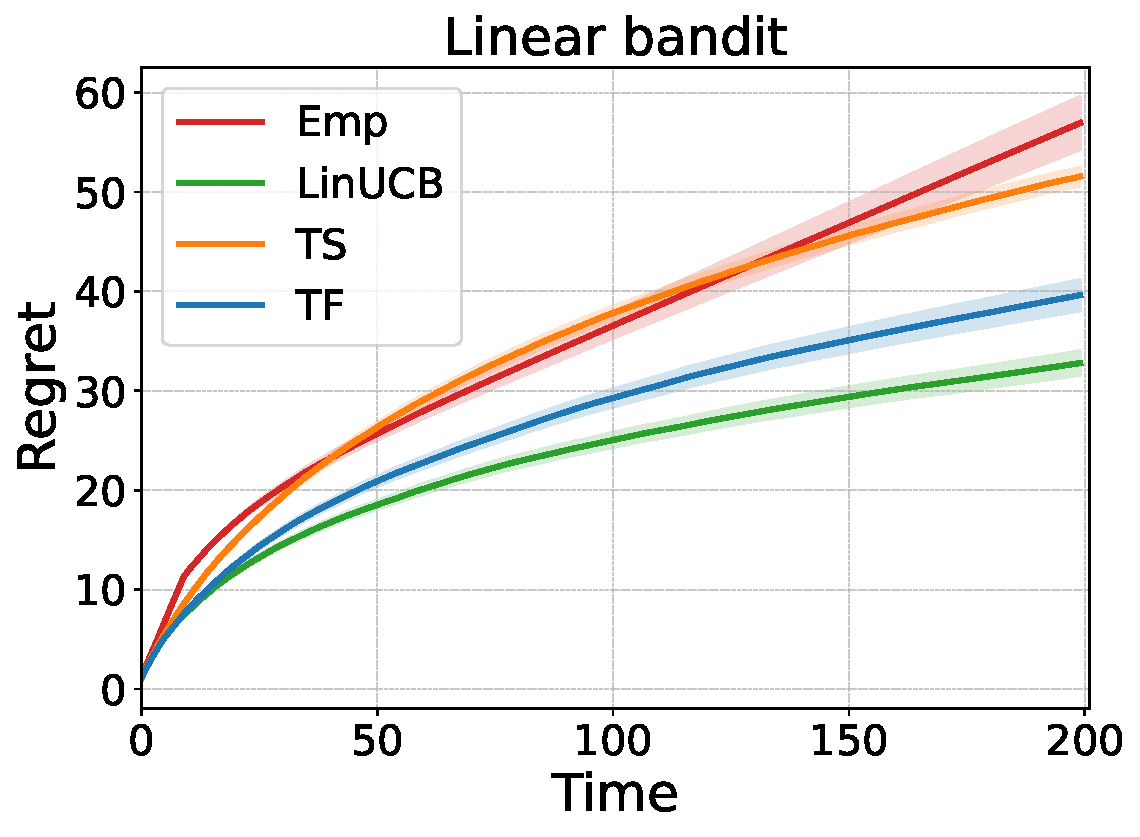
\includegraphics[width=0.35\linewidth]{Sections/figs/record_2_cum_True.pdf}
\hspace{2em}
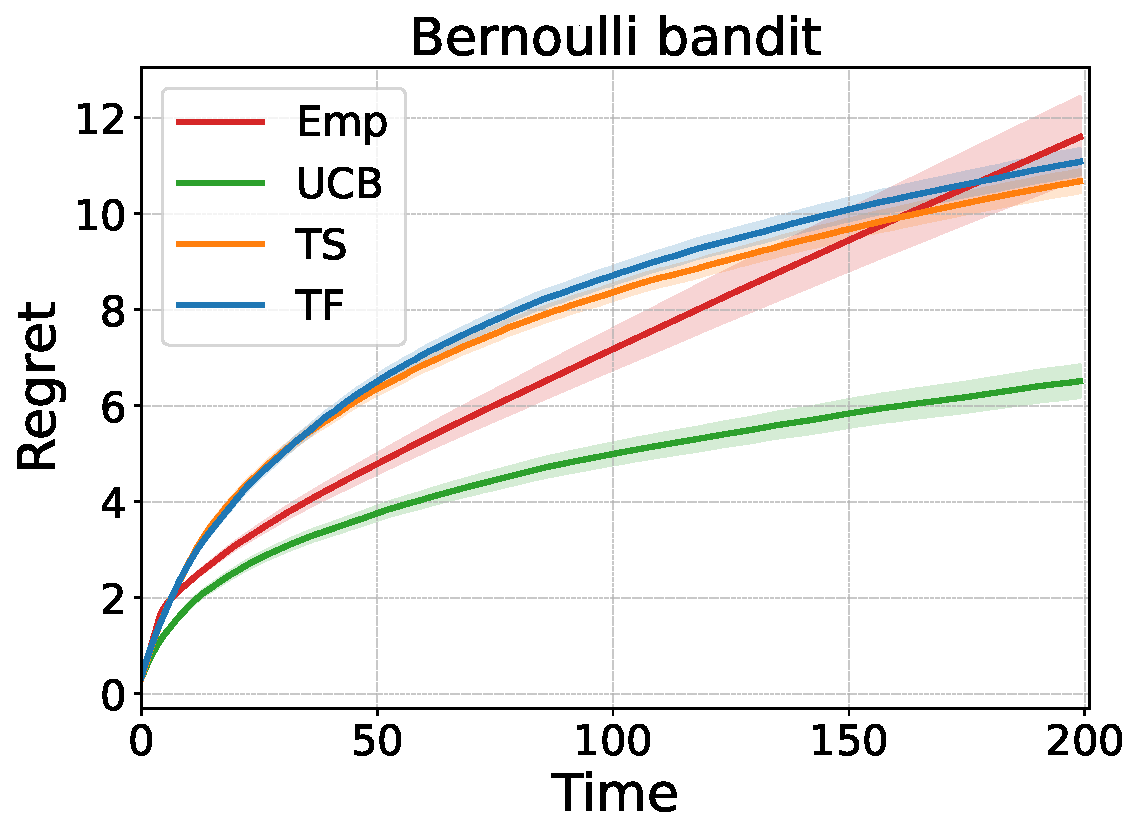
\includegraphics[width=0.35\linewidth]{Sections/figs/record_1_cum_True.pdf}
\vspace{-1em}
\caption{Regrets of transformer (TF), empirical average (Emp), Thompson sampling (TS) and LinUCB or UCB (LinUCB reduces to UCB for Bernoulli bandits). Left: linear bandit with $d=5$, $A=10$, $\sigma=1.5$, $\sAlg_0=\sAlg_\shortexp=\LinUCB$. Right: Bernoulli bandit with $d=5$, $\sAlg_0=(\sAlg_{\mathrm{unif}}+\sAlg_{\TS})/2$ and $\sAlg_\shortexp=\action^*$. The simulation is repeated 500 times. Shading displays the standard deviation of the regret estimates. } 
\label{fig:regret_1} 
\end{figure}


\section{Conclusions}

This paper theoretically investigates the ICRL capability of supervised-pretrained transformers. We demonstrate how transformers can efficiently implement prevalent RL algorithms including LinUCB, Thompson sampling, and UCB-VI, achieving near-optimal regrets in respective settings. We also provide sample complexity guarantees for the supervised pretraining approach to learning these algorithms. The generalization error scales with the covering number of the transformer class as well as the distribution ratio between the expert and offline algorithms. Simulations validate our theoretical findings.  
Finally, we discuss the limitations of our results and provide additional discussions in Appendix~\ref{sec:limitation}.





\section*{Acknowledgement}

The authors would like to thank Peter L. Bartlett for the valuable discussions, and Jonathan Lee for the valuable discussions regarding Decision-Pretrained Transformers as well as providing an early version of its implementation. This work is supported by NSF CCF-2315725, DMS-2210827, NSF Career award DMS-2339904, and an Amazon Research Award.
% \clearpage
\bibliography{references}
\bibliographystyle{plainnat}
\end{document}
